\documentclass[PianoDiQualifica.tex]{subfiles}

\begin{document}

\section{Test}
Al fine di produrre \gl{software} di qualità, il gruppo ha strutturato dei test atti a verificare che le funzionalità del software \gl{prodotto} corrispondano alle attese.
Tali test sono ottenuti dall'applicazione delle tecniche di analisi dinamica descritte nel documento \NPdocRP{}. Inoltre, devono possedere le seguenti caratteristiche:
\begin{itemize}
	\item devono essere ripetibili al fine di fornire informazioni utili per poter eseguire operazioni di correzione, ove sia necessario;
	\item devono essere tracciabili al fine di classificare le informazioni ottenute per garantire una più facile consultazione;
\end{itemize}
Le tipologie di test che verranno eseguiti sono:
\begin{itemize}
\item \textbf{Test di \gl{validazione}:} test che hanno lo scopo di verificare che tutte le funzionalità richieste dal \gl{proponente} siano soddisfatte. A questo scopo, attraverso una serie di
azioni, si andrà a simulare il comportamento generale del software e dell'utente che interagisce con esso;
\item \textbf{Test di unità: } test che  hanno lo scopo di verificare il corretto funzionamento delle unità. Le unità, individuate durante la fase di progettazione, sono le
		più piccole parti del \gl{sistema} dotate di funzionamento proprio. Questo si traduce nel verificare metodi e classi scritte dai \PRP{};
\item \textbf{Test di integrazione: } test che hanno lo scopo di verificare il corretto funzionamento delle varie componenti. In particolare, l'obiettivo è quello di testare le varie componenti prodotte dall'unione delle unità. Nel determinarli, è stato scelto l'approccio top-down, in maniera tale da sottoporre per prime le componenti di livello più alto ai test, integrandole fin da subito. Così facendo anche la logica di alto livello e il flusso di dati vengono sottoposti a test fin da subito; sarà perciò necessario simulare le componenti di livello più basso con degli stub. Una volta codificate, le componenti di più basso livello dovranno a loro volta essere
integrate e testate. In questo modo, i difetti rilevati dai test saranno spesso attribuiti all'ultima componente aggiunta. In \DPdoc{} sono descritte come le componenti devono interagire tra loro;
\item \textbf{Test di sistema: }test che hanno lo scopo di verificare il corretto funzionamento del prodotto software. Inoltre verranno verificate la sua robustezza in presenza di
		possibili malfunzionamenti e il suo comportamento di fronte a possibili violazioni;
\item \textbf{Test di regressione: } test che hanno lo scopo di verificare che una modifica dell'implementazione del software non ne comprometta la qualità. Consistono nella ripetizione di test di unità o integrazione sul componente modificato.			
\end{itemize}

Per la definizione ed esecuzione dei test il gruppo ha deciso di adottare il \textbf{Modello a V}.

\begin{figure}[htbp]
	\centering
	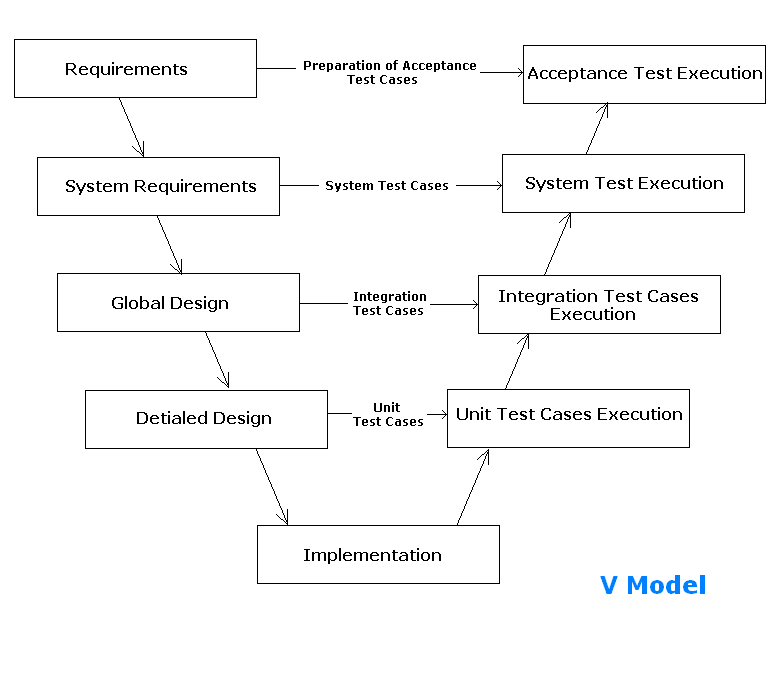
\includegraphics[height=6cm,width=5cm]{v-model.png}
	\caption{Modello a V}
\end{figure}

Questo modello prevede che le attività di testing inizino prima del periodo di codifica e che esse siano tracciate a requisiti e componenti di progettazione. 
Questo rigore comporta un maggiore risparmio di risorse in quanto nulla di quello che viene definito risulta essere non necessario.




	\paragraph{Test di Validazione}
I test di \gl{validazione} saranno identificati secondo quanto riportato nel documento \NPdoc{}.
\normalsize
\begin{longtable}{|c|>{}m{8cm}|c|}
\hline
\textbf{Id Test} & \textbf{Descrizione} & \textbf{Stato}\\
\hline
\endhead
\hypertarget{TVFO1}{TVFO1} & L'utente deve \gl{verifica}re che il \gl{sistema} riesca a riconoscerlo come ospite o possibile amministratore. All'utente viene richiesto di:
\begin{itemize}
\item fornire nome e cognome;
\end{itemize} & \textit{Non Implementato}\\ \hline
\hypertarget{TVFO1.1.2}{TVFO1.1.2} & L'utente deve verificare che il sistema ne permetta l'accesso all'area amministrativa tramite l'assistente virtuale. All'utente viene richiesto di:
\begin{itemize}
\item comunicare i propri dati identificativi;
\item verificare che il sistema riconosca l'utente come un possibile amministratore non autenticato;
\item comunicare l'intento di volersi autenticare come amministratore;
\item comunicare la frase per lo \gl{Speaker Recognition};
\item verificare l'accesso all'area amministrativa.
\end{itemize} & \textit{Non Implementato}\\ \hline
\hypertarget{TVFO2.1}{TVFO2.1} & L'utente deve verificare che il sistema permetta la creazione di una nuova \gl{direttiva}. All'utente viene richiesto di:
\begin{itemize}
\item autenticarsi come amministratore;
\item comunicare l'intento di voler creare una nuova direttiva;
\item inserire il nome della direttiva;
\item inserire la funzione della direttiva;
\item inserire il target della direttiva;
\item confermare la creazione della direttiva;
\item verificare che la direttiva sia stata creata correttamente.
\end{itemize}
 & \textit{Non Implementato}\\ \hline
\hypertarget{TVFO2.1.1.6}{TVFO2.1.1.6} & L'utente deve verificare che, durante la creazione di una direttiva, l'inserimento di dati non validi (funzione o target della direttiva inesistenti) comporti la visualizzazione di un messaggio d'errore. All'utente viene richiesto di:
\begin{itemize}
\item autenticarsi come amministratore;
\item comunicare l'intento di voler creare una nuova direttiva;
\item inserire il nome della direttiva;
\item inserire una funzione per la direttiva che non sia valida (inesistente);
\item inserire un target per la direttiva che non sia valido (inesistente);
\item verificare la comparsa di un messaggio d'errore.
\end{itemize} & \textit{Non Implementato}\\ \hline
\hypertarget{TVFO2.1.2}{TVFO2.1.2} & L'utente deve verificare che il sistema permetta l'eliminazione di una direttiva. All'utente viene richiesto di:
\begin{itemize}
\item autenticarsi come amministratore;
\item comunicare l'intento di voler eliminare una direttiva;
\item comunicare il nome della direttiva da eliminare;
\item confermare l'eliminazione della direttiva;
\item verificare che la direttiva sia stata eliminata correttamente.
\end{itemize}
 & \textit{Non Implementato}\\ \hline
\hypertarget{TVFO2.1.4}{TVFO2.1.4} & L'utente deve verificare che il sistema permetta la visualizzazione di una direttiva. All'utente viene richiesto di:
\begin{itemize}
\item autenticarsi come amministratore;
\item comunicare l'intento di voler visualizzare una direttiva;
\item verificare che il sistema permetta la visualizzazione di nome, funzione, target,funzionalità e abilitazione della direttiva.
\end{itemize} & \textit{Non Implementato}\\ \hline
\hypertarget{TVFO2.2}{TVFO2.2} & L'utente deve verificare che il sistema permetta la modifica dei dati del proprio profilo. All'utente viene richiesto di:
\begin{itemize}
\item autenticarsi come amministratore;
\item comunicare l'intento di voler modificare il proprio profilo;
\item comunicare nome e cognome;
\item confermare la modifica;
\item verificare che la modifica sia stata effettuata;
\end{itemize}
 & \textit{Non Implementato}\\ \hline
\hypertarget{TVFO3.1}{TVFO3.1} & L'utente deve verificare che sia possibile comunicare al sistema la persona che si desidera incontrare. All'utente viene richiesto di:
\begin{itemize}
\item aver comunicato i propri dati al sistema ed essere riconosciuti come ospiti;
\item comunicare la persona che si desidera raggiungere;
\item verificare che il sistema abbia capito le informazioni comunicate;
\end{itemize} & \textit{Non Implementato}\\ \hline
\hypertarget{TVFO5}{TVFO5} & L'utente deve verificare che, nel caso in cui il sistema nel caso non riesca ad interpretare la risposta, chieda nuovamente l'informazione all'utente. All'utente viene richiesto di:
\begin{itemize}
\item comunicare al sistema qualcosa che non può essere interpretato da esso;
\item verificare che il sistema richieda nuovamente l'informazione.
\end{itemize} & \textit{Non Implementato}\\ \hline
\hypertarget{TVFO7}{TVFO7} & L'utente deve verificare che, nel caso in cui esso sia già stato un ospite in passato, il sistema lo riconosca. All'utente viene richiesto di:
\begin{itemize}
\item aver comunicato i propri dati al sistema ed essere riconosciuti come ospiti;
\item verificare che il sistema riconosca l'utente come qualcuno che è già stato un ospite in passato.
\end{itemize}
 & \textit{Non Implementato}\\ \hline
\caption[Test di Validazione]{Test di Validazione}
\label{tabella:test0}
\end{longtable}
\clearpage

\paragraph{Test di Sistema}
I test di sistema saranno identificati secondo quanto riportato nel documento \NPdoc{}.
\normalsize
\begin{longtable}{|c|>{}m{8cm}|c|}
\hline
\textbf{Id Test} & \textbf{Descrizione} & \textbf{Stato}\\
\hline
\endhead
\hypertarget{TSFO1}{TSFO1} & Il sistema deve poter riconoscere un utente come ospite. & \textit{Non Implementato}\\ \hline
\hypertarget{TSFO1.1.2.1}{TSFO1.1.2.1} & Il sistema deve permettere all'utente di autenticarsi come amministratore tramite frase di riconoscimento. & \textit{Non Implementato}\\ \hline
\hypertarget{TSFO2.1.1}{TSFO2.1.1} & Il sistema deve permettere all'amministratore di poter creare una nuova direttiva. & \textit{Non Implementato}\\ \hline
\hypertarget{TSFO2.1.2}{TSFO2.1.2} & Il sistema deve permettere all'amministratore di poter eliminare una direttiva di cui ha i privilegi. & \textit{Non Implementato}\\ \hline
\hypertarget{TSFO2.1.4}{TSFO2.1.4} & Il sistema deve permettere all'amministratore di poter visualizzare le \gl{direttive} di cui ha i privilegi. & \textit{Non Implementato}\\ \hline
\hypertarget{TSFO2.2.1}{TSFO2.2.1} & L'amministratore deve poter modificare il nome e cognome del suo profilo. & \textit{Non Implementato}\\ \hline
\hypertarget{TSFO3.1}{TSFO3.1} & Il sistema deve permettere all'ospite di richiedere la persona desiderata. & \textit{Non Implementato}\\ \hline
\hypertarget{TSFO5}{TSFO5} & Il sistema deve richiedere nuovamente le informazioni nel caso in cui non fossero state comprese. & \textit{Non Implementato}\\ \hline
\hypertarget{TSFO7}{TSFO7} & Il sistema deve essere in grado di riconoscere ospiti già stati in visita all'azienda. In questo caso, l'assistente virtuale deve poter prevedere le sue necessità. & \textit{Non Implementato}\\ \hline
\hypertarget{TSFO8}{TSFO8} & Il sistema deve sollecitare la persona desiderata o eventualmente avvisare gli altri membri dell'azienda su richiesta dell'ospite. & \textit{Non Implementato}\\ \hline
\hypertarget{TSFO13}{TSFO13} & Il sistema deve comunicare nell'opportuno canale di \gl{Slack} le informazioni raccolte durante l'interazione con l'ospite. & \textit{Non Implementato}\\ \hline
\hypertarget{TSVO1.1}{TSVO1.1} & Vogliamo testare che il \gl{software} funzioni correttamente in un PC con sistema operativo Windows 7 o superiore.
 & \textit{Non Implementato}\\ \hline
\hypertarget{TSVO4}{TSVO4} & Le pagine HTML devono essere validate. & \textit{Non Implementato}\\ \hline
\hypertarget{TSVO5}{TSVO5} & I fogli di stile CSS devono essere validati. & \textit{Non Implementato}\\ \hline
\hypertarget{TSVO10}{TSVO10} & Vogliamo testare che il software funzioni correttamente con il \gl{browser} Google Chrome versione 53 o superiore. & \textit{Non Implementato}\\ \hline
\caption[Test di Sistema]{Test di Sistema}
\label{tabella:test1}
\end{longtable}
\clearpage

\paragraph{Test di Integrazione}
I test di integrazione saranno identificati secondo quanto riportato nel documento \NPdoc{}.
\normalsize
\begin{longtable}{|c|>{}m{8cm}|c|}
\hline
\textbf{Id Test} & \textbf{Descrizione} & \textbf{Stato}\\
\hline
\endhead
\hypertarget{TI1}{TI1} & Vogliamo verificare che \file{Recorder}, \file{Logic}, \file{Utility}, \file{TTS}, \file{ConversationApp} e \file{ApplicationManager} interagiscano correttamente fra loro. & \textit{Non Implementato}\\ \hline
\hypertarget{TI2}{TI2} & Vogliamo verificare che \file{APIGateway}, \file{STT}, \file{VirtualAssistant},  \file{Users}, \file{Guests}, \file{Rules}, \file{Members}, \file{Conversations} e \file{Events} interagiscano correttamente tra di loro. Inoltre, vogliamo verificare che interagiscano correttamente con i servizi e librerie esterne AWS, Speaker Recognition, \gl{Speech to text} IBM Watson, api.ai, Slack e \file{WebAPI}. & \textcolor{green}{\textit{Superato}}\\ \hline
\hypertarget{TI3}{TI3} & Vogliamo verificare che le seguenti classi, contenute in \file{Client::ApplicationManager}, interagiscano tra loro correttamente: \file{ApplicationManagerObserver}, \file{ApplicationRegistryClient}, \file{ApplicationRegistryLocalClient}, \file{ApplicationLocalRegistry}, \file{Manager}, \file{State}, \file{Application}, \file{ApplicationPackage}. & \textcolor{green}{\textit{Superato}}\\ \hline
\hypertarget{TI4}{TI4} & Vogliamo verificare che le seguenti classi, contenute in \file{Client::Logic}, interagiscano tra loro correttamente: \file{DataArrivedSubject}, \file{DataArrivedObservable}, \file{Logic}, \file{HttpError}, \file{HttpPromise}, \file{LogicObserver}. & \textit{Non Implementato}\\ \hline
\hypertarget{TI5}{TI5} & Vogliamo verificare che le seguenti classi, contenute in \file{Client::Recorder}, interagiscano tra loro correttamente: \file{Recorder}, \file{RecorderWorker}, \file{RecorderMsg}, \file{RecorderWorkerMsg}, \file{RecorderWorkerConfig}, \file{RecorderConfig}, \file{SpeechEndSubject}, \file{SpeechEndObservable}. & \textcolor{green}{\textit{Superato}}\\ \hline
\hypertarget{TI6}{TI6} & Vogliamo verificare che le seguenti classi, contenute in \file{Client::TTS}, interagiscano tra loro correttamente: \file{TTSConfig}, \file{Player}, \file{PlayerObserver}. & \textcolor{green}{\textit{Superato}}\\ \hline
\hypertarget{TI7}{TI7} & Vogliamo verificare che le seguenti classi, contenute in \file{Client::Utility}, interagiscano tra loro correttamente: \file{BoolSubject}, \file{BoolObservable}, \file{BoolObserver}. & \textcolor{green}{\textit{Superato}}\\ \hline
\hypertarget{TI8}{TI8} & Vogliamo verificare che le seguenti classi, contenute in \file{Back-end::APIGateway}, interagiscano tra loro correttamente: \file{VocalAPI}, \file{Enrollement}. & \textcolor{green}{\textit{Superato}}\\ \hline
\hypertarget{TI9}{TI9} & Vogliamo verificare che le seguenti classi, contenute in \file{Back-end::Users}, interagiscano tra loro correttamente: \file{UsersDAODynamoDB}, \file{User}, \file{UsersService}. & \textcolor{green}{\textit{Superato}}\\ \hline
\hypertarget{TI10}{TI10} & Vogliamo verificare che le seguenti classi, contenute in \file{Back-end::Rules}, interagiscano tra loro correttamente: \file{Rule}, \file{RulesDAODynamoDB}, \file{RuleTarget}, \file{RuleTaskInstance}, \file{RulesService}, \file{TasksDAODynamoDB}, \file{Task}. & \textcolor{green}{\textit{Superato}}\\ \hline
\hypertarget{TI11}{TI11} & Vogliamo verificare che le seguenti classi, contenute in \file{Back-end::VirtualAssistant}, interagiscano tra loro correttamente: \file{VAService}, \file{ApiAIVAAdapter}, \file{VAQuery}, \file{Agent}, \file{AgentDAODynamoDB}, \file{VAEventObject}, \file{Fulfillment}, \file{MsgObject}, \file{ButtonObject}. & \textcolor{green}{\textit{Superato}}\\ \hline
\hypertarget{TI12}{TI12} & Vogliamo verificare che le seguenti classi, contenute in \file{Back-end::Member}, interagiscano tra loro correttamente: \file{MembersSlackDAO}, \file{Member}. & \textcolor{green}{\textit{Superato}}\\ \hline
\hypertarget{TI13}{TI13} & Vogliamo verificare che le seguenti classi, contenute in \file{Back-end::Guests}, interagiscano tra loro correttamente: \file{Guest}, \file{GuestDAODynamoDB}. & \textcolor{green}{\textit{Superato}}\\ \hline
\hypertarget{TI14}{TI14} & Vogliamo verificare che le seguenti classi, contenute in \file{Back-end::Conversations}, interagiscano tra loro correttamente: \file{ConversationDAODynamoDB}, \file{Conversation}, \file{ConversationMsg}.
 & \textcolor{green}{\textit{Superato}}\\ \hline
\hypertarget{TI15}{TI15} & Vogliamo verificare che le seguenti classi, contenute in \file{Back-end::Events}, interagiscano tra loro correttamente: \file{SNSRecord}, \file{SNSMessage}.
 & \textcolor{green}{\textit{Superato}}\\ \hline
\hypertarget{TI16}{TI16} & Vogliamo verificare che le seguenti classi, contenute in \file{Back-end::Notifications}, interagiscano tra loro correttamente: \file{NotificationChannel}, \file{Purpose}, \file{Topic}, \file{NotificationMessage}, \file{Attachment}, \file{Action}, \file{ConfirmationFields}. & \textcolor{green}{\textit{Superato}}\\ \hline
\hypertarget{TI17}{TI17} & Vogliamo verificare che le seguenti classi, contenute in \file{Back-end::Utility}, interagiscano tra loro correttamente: \file{WebhookRequest}, \file{ProcessingResult}, \file{LamdaIdEvent}, \file{PathIdParam}. & \textcolor{green}{\textit{Superato}}\\ \hline
\hypertarget{TI18}{TI18} & Vogliamo verificare che le seguenti classi, contenute in \file{Client::ConversationApp}, interagiscano tra loro correttamente: \file{ConversationApp}, \file{ConversationActionObserver}, \file{ConversationActionObservable}, \file{ConversaionActionSubject}, \file{ConversationAction}, \file{ConversationDispatcher}, \file{ConversationView}, \file{MessageStore}. & \textcolor{green}{\textit{Superato}}\\ \hline
\caption[Test di Integrazione]{Test di Integrazione}
\label{tabella:test2}
\end{longtable}
\clearpage

\paragraph{Test di Unità}
I test di unita saranno identificati secondo quanto riportato nel documento \NPdoc{}.
\normalsize
\begin{longtable}{|c|>{}m{8cm}|c|}
\hline
\textbf{Id Test} & \textbf{Descrizione} & \textbf{Stato}\\
\hline
\endhead
\hypertarget{TU1}{TU1} & Vogliamo testare che il metodo imposti il campo \file{status} della risposta a 200 e che il campo \file{speech} sia uguale al campo \file{fulfillment.speech} del corpo della richiesta, in caso il token sia presente e valido. & \textcolor{green}{\textit{Superato}}\\ \hline
\hypertarget{TU2}{TU2} & Vogliamo testare che il metodo imposti il campo \file{status} della risposta a 403 in caso di mancata autenticazione, ovvero token assente o non valido. & \textcolor{green}{\textit{Superato}}\\ \hline
\hypertarget{TU3}{TU3} & Vogliamo testare che il metodo sollevi un'eccezione alla sua chiamata. & \textcolor{green}{\textit{Superato}}\\ \hline
\hypertarget{TU4}{TU4} & Vogliamo testare che il metodo accetti un parametro di tipo \file{Agent} senza generare eccezioni. & \textcolor{green}{\textit{Superato}}\\ \hline
\hypertarget{TU5}{TU5} & Vogliamo testare che il metodo sollevi un'eccezione nel caso in cui il parametro non sia di tipo \file{Agent}. & \textcolor{green}{\textit{Superato}}\\ \hline
\hypertarget{TU6}{TU6} & Vogliamo testare che, se la chiamata al servizio di STT non va a buon fine, venga chiamato il metodo \file{succeed} del \file{context}, con un parametro \file{LambdaResponse} avente \file{statusCode} pari a 500. & \textcolor{green}{\textit{Superato}}\\ \hline
\hypertarget{TU7}{TU7} & Vogliamo testare che, se lo \file{status} della risposta ricevuta dall'assistente virtuale è diverso da 200, venga chiamato il metodo \file{succeed} di \file{context} con un oggetto di tipo \file{LambdaResponse} come parametro, avente il campo \file{statusCode} uguale a quello ricevuto e corpo del messaggio "Errore nel contattare l'assistente virtuale". & \textcolor{green}{\textit{Superato}}\\ \hline
\hypertarget{TU8}{TU8} & Vogliamo testare che, se l'action del body della risposta è uguale a \file{"rule.add"}, venga chiamato il metodo privato \file{addRule}. & \textcolor{green}{\textit{Superato}}\\ \hline
\hypertarget{TU9}{TU9} & Vogliamo testare che, se l'action del body della risposta è uguale a \file{"user.add"}, venga chiamato il metodo privato \file{addUser}. & \textcolor{green}{\textit{Superato}}\\ \hline
\hypertarget{TU10}{TU10} & Vogliamo testare che, se l'action del body della risposta è uguale a \file{"user.addEnrollment"}, venga chiamato il metodo privato \file{addUserEnrollment}. & \textcolor{green}{\textit{Superato}}\\ \hline
\hypertarget{TU11}{TU11} & Vogliamo testare che, se l'action del body della risposta è uguale a \file{"rule.get"}, venga chiamato il metodo privato \file{getRule}. & \textcolor{green}{\textit{Superato}}\\ \hline
\hypertarget{TU12}{TU12} & Vogliamo testare che, se l'action del body della risposta è uguale a \file{"rule.getList"}, venga chiamato il metodo privato \file{getRuleList}. & \textcolor{green}{\textit{Superato}}\\ \hline
\hypertarget{TU13}{TU13} & Vogliamo testare che, se l'action del body della risposta è uguale a \file{"user.get"}, venga chiamato il metodo privato \file{getUser}. & \textcolor{green}{\textit{Superato}}\\ \hline
\hypertarget{TU14}{TU14} & Vogliamo testare che, se l'action del body della risposta è uguale a \file{"user.login"}, venga chiamato il metodo privato \file{loginUser}. & \textcolor{green}{\textit{Superato}}\\ \hline
\hypertarget{TU15}{TU15} & Vogliamo testare che, se l'action del body della risposta è uguale a \file{"rule.remove"}, venga chiamato il metodo privato \file{removeRule}. & \textcolor{green}{\textit{Superato}}\\ \hline
\hypertarget{TU16}{TU16} & Vogliamo testare che, se l'action del body della risposta è uguale a \file{"user.remove"}, venga chiamato il metodo privato \file{removeUser}. & \textcolor{green}{\textit{Superato}}\\ \hline
\hypertarget{TU17}{TU17} & Vogliamo testare che, se l'action del body della risposta è uguale a \file{"user.resetEnrollment"}, venga chiamato il metodo privato \file{resetUserEnrollment}. & \textcolor{green}{\textit{Superato}}\\ \hline
\hypertarget{TU18}{TU18} & Vogliamo testare che, se l'action del body della risposta è uguale a \file{"rule.update"}, venga chiamato il metodo privato \file{updateRule}. & \textcolor{green}{\textit{Superato}}\\ \hline
\hypertarget{TU19}{TU19} & Vogliamo testare che, se l'action del body della risposta è uguale a \file{"user.update"}, venga chiamato il metodo privato \file{updateUser}. & \textcolor{green}{\textit{Superato}}\\ \hline
\hypertarget{TU20}{TU20} & Vogliamo testare che, se durante la chiamata al metodo privato \file{addRule} si verifica un errore, venga chiamato il metodo \file{succeed} del \file{context} con un parametro \file{LambdaResponse} il quale campo \file{statusCode} è impostato ad un valore uguale a quello restituito dal microservizio \file{Rules}. & \textcolor{green}{\textit{Superato}}\\ \hline
\hypertarget{TU21}{TU21} & Vogliamo testare che, se durante la chiamata al metodo privato \file{addUser} si verifica un errore, venga chiamato il metodo \file{succeed} del \file{context} con un parametro \file{LambdaResponse} il quale campo \file{statusCode} è impostato ad un valore uguale a quello restituito dal \gl{microservizio} \file{Users}. & \textcolor{green}{\textit{Superato}}\\ \hline
\hypertarget{TU22}{TU22} & Vogliamo testare che, se durante la chiamata al metodo privato \file{addUserEnrollment} si verifica un errore, venga chiamato il metodo \file{succeed} del \file{context} con un parametro \file{LambdaResponse} il quale campo \file{statusCode} è impostato ad un valore uguale a quello restituito dal microservizio \file{Users}. & \textcolor{green}{\textit{Superato}}\\ \hline
\hypertarget{TU23}{TU23} & Vogliamo testare che, se durante la chiamata al metodo privato \file{getRule} si verifica un errore, venga chiamato il metodo \file{succeed} del \file{context} con un parametro \file{LambdaResponse} il quale campo \file{statusCode} è impostato ad un valore uguale a quello restituito dal microservizio \file{Rules}. & \textcolor{green}{\textit{Superato}}\\ \hline
\hypertarget{TU24}{TU24} & Vogliamo testare che, se durante la chiamata al metodo privato \file{getRuleList} si verifica un errore, venga chiamato il metodo \file{succeed} del \file{context} con un parametro \file{LambdaResponse} il quale campo \file{statusCode} è impostato ad un valore uguale a quello restituito dal microservizio \file{Rules}. & \textcolor{green}{\textit{Superato}}\\ \hline
\hypertarget{TU25}{TU25} & Vogliamo testare che, se durante la chiamata al metodo privato \file{getUser} si verifica un errore, venga chiamato il metodo \file{succeed} del \file{context} con un parametro \file{LambdaResponse} il quale campo \file{statusCode} è impostato ad un valore uguale a quello restituito dal microservizio \file{Users}. & \textcolor{green}{\textit{Superato}}\\ \hline
\hypertarget{TU26}{TU26} & Vogliamo testare che, se durante la chiamata al metodo privato \file{getUserList} si verifica un errore, venga chiamato il metodo \file{succeed} del \file{context} con un parametro \file{LambdaResponse} il quale campo \file{statusCode} è impostato ad un valore uguale a quello restituito dal microservizio \file{Users}. & \textcolor{green}{\textit{Superato}}\\ \hline
\hypertarget{TU27}{TU27} & Vogliamo testare che, se durante la chiamata al metodo privato \file{loginUser} si verifica un errore, venga chiamato il metodo \file{succeed} del \file{context} con un parametro \file{LambdaResponse} il quale campo \file{statusCode} è impostato ad un valore uguale a quello restituito dal microservizio \file{Users}. & \textcolor{green}{\textit{Superato}}\\ \hline
\hypertarget{TU28}{TU28} & Vogliamo testare che, se durante la chiamata al metodo privato \file{removeRule} si verifica un errore, venga chiamato il metodo \file{succeed} del \file{context} con un parametro \file{LambdaResponse} il quale campo \file{statusCode} è impostato ad un valore uguale a quello restituito dal microservizio \file{Rules}. & \textcolor{green}{\textit{Superato}}\\ \hline
\hypertarget{TU29}{TU29} & Vogliamo testare che, se durante la chiamata al metodo privato \file{removeUser} si verifica un errore, venga chiamato il metodo \file{succeed} del \file{context} con un parametro \file{LambdaResponse} il quale campo \file{statusCode} è impostato ad un valore uguale a quello restituito dal microservizio \file{Users}. & \textcolor{green}{\textit{Superato}}\\ \hline
\hypertarget{TU30}{TU30} & Vogliamo testare che, se durante la chiamata al metodo privato \file{resetUserEnrollment} si verifica un errore, venga chiamato il metodo \file{succeed} del \file{context} con un parametro \file{LambdaResponse} il quale campo \file{statusCode} è impostato ad un valore uguale a quello restituito dal microservizio \file{Users}. & \textcolor{green}{\textit{Superato}}\\ \hline
\hypertarget{TU31}{TU31} & Vogliamo testare che, se durante la chiamata al metodo privato \file{updateRule} si verifica un errore, venga chiamato il metodo \file{succeed} del \file{context} con un parametro \file{LambdaResponse} il quale campo \file{statusCode} è impostato ad un valore uguale a quello restituito dal microservizio \file{Rules}. & \textcolor{green}{\textit{Superato}}\\ \hline
\hypertarget{TU32}{TU32} & Vogliamo testare che, se durante la chiamata al metodo privato \file{updateUser} si verifica un errore, venga chiamato il metodo \file{succeed} del \file{context} con un parametro \file{LambdaResponse} il quale campo \file{statusCode} è impostato ad un valore uguale a quello restituito dal microservizio \file{Users}. & \textcolor{green}{\textit{Superato}}\\ \hline
\hypertarget{TU33}{TU33} & Vogliamo testare che, se la risposta ricevuta dalla chiamata al microservizio \file{Rules} ha uno status code diverso da 200, il metodo sollevi un'eccezione di tipo \file{Exception} con campo \file{code} pari allo status code della risposta. & \textcolor{green}{\textit{Superato}}\\ \hline
\hypertarget{TU34}{TU34} & Vogliamo testare che, se la risposta ricevuta dalla chiamata al microservizio \file{Users} ha uno status code diverso da 200, il metodo sollevi un'eccezione di tipo \file{Exception} con campo \file{code} pari allo status code della risposta. & \textcolor{green}{\textit{Superato}}\\ \hline
\hypertarget{TU35}{TU35} & Vogliamo testare che, se la risposta ricevuta dalla chiamata al microservizio \file{Users} ha uno status code diverso da 200, il metodo sollevi un'eccezione di tipo \file{Exception} con campo \file{code} pari allo status code della risposta. & \textcolor{green}{\textit{Superato}}\\ \hline
\hypertarget{TU36}{TU36} & Vogliamo testare che, se la risposta ricevuta dalla chiamata al microservizio \file{Rules} ha uno status code diverso da 200, il metodo sollevi un'eccezione di tipo \file{Exception} con campo \file{code} pari allo status code della risposta. & \textcolor{green}{\textit{Superato}}\\ \hline
\hypertarget{TU37}{TU37} & Vogliamo testare che, se la risposta ricevuta dalla chiamata al microservizio \file{Rules} ha uno status code diverso da 200, il metodo sollevi un'eccezione di tipo \file{Exception} con campo \file{code} pari allo status code della risposta. & \textcolor{green}{\textit{Superato}}\\ \hline
\hypertarget{TU38}{TU38} & Vogliamo testare che, se la risposta ricevuta dalla chiamata al microservizio \file{Users} ha uno status code diverso da 200, il metodo sollevi un'eccezione di tipo \file{Exception} con campo \file{code} pari allo status code della risposta. & \textcolor{green}{\textit{Superato}}\\ \hline
\hypertarget{TU39}{TU39} & Vogliamo testare che, se la risposta ricevuta dalla chiamata al microservizio \file{Users} ha uno status code diverso da 200, il metodo sollevi un'eccezione di tipo \file{Exception} con campo \file{code} pari allo status code della risposta. & \textcolor{green}{\textit{Superato}}\\ \hline
\hypertarget{TU40}{TU40} & Vogliamo testare che, se la risposta ricevuta dalla chiamata al microservizio \file{Users} ha uno status code diverso da 200, il metodo sollevi un'eccezione di tipo \file{Exception} con campo \file{code} pari allo status code della risposta. & \textcolor{green}{\textit{Superato}}\\ \hline
\hypertarget{TU41}{TU41} & Vogliamo testare che, se la risposta ricevuta dalla chiamata al microservizio \file{Rules} ha uno status code diverso da 200, il metodo sollevi un'eccezione di tipo \file{Exception} con campo \file{code} pari allo status code della risposta. & \textcolor{green}{\textit{Superato}}\\ \hline
\hypertarget{TU42}{TU42} & Vogliamo testare che, se la risposta ricevuta dalla chiamata al microservizio \file{Users} ha uno status code diverso da 200, il metodo sollevi un'eccezione di tipo \file{Exception} con campo \file{code} pari allo status code della risposta. & \textcolor{green}{\textit{Superato}}\\ \hline
\hypertarget{TU43}{TU43} & Vogliamo testare che, se la risposta ricevuta dalla chiamata al microservizio \file{Users} ha uno status code diverso da 200, il metodo sollevi un'eccezione di tipo \file{Exception} con campo \file{code} pari allo status code della risposta. & \textcolor{green}{\textit{Superato}}\\ \hline
\hypertarget{TU44}{TU44} & Vogliamo testare che, se la risposta ricevuta dalla chiamata al microservizio \file{Rules} ha uno status code diverso da 200, il metodo sollevi un'eccezione di tipo \file{Exception} con campo \file{code} pari allo status code della risposta. & \textcolor{green}{\textit{Superato}}\\ \hline
\hypertarget{TU45}{TU45} & Vogliamo testare che, se la risposta ricevuta dalla chiamata al microservizio \file{Users} ha uno status code diverso da 200, il metodo sollevi un'eccezione di tipo \file{Exception} con campo \file{code} pari allo status code della risposta. & \textcolor{green}{\textit{Superato}}\\ \hline
\hypertarget{TU46}{TU46} & Vogliamo dimostrare che, se la chiamata al metodo \file{sns.publish} genera un errore, venga chiamato il metodo \file{succeed} del \file{context} con un parametro \file{LambdaResponse} avente campo \file{statusCode} pari allo \file{status} dell'errore. & \textcolor{green}{\textit{Superato}}\\ \hline
\hypertarget{TU47}{TU47} & Vogliamo testare che, se lo status code della risposta di un microservizio è pari a 200 e l'action contenuta nel suo body non corrisponde a nessuna action supportata dal back-end, il metodo rielabori la risposta e la inoltri. & \textcolor{green}{\textit{Superato}}\\ \hline
\hypertarget{TU48}{TU48} & Vogliamo testare che il metodo accetti un parametro di tipo \file{Conversation} senza generare eccezioni. & \textcolor{green}{\textit{Superato}}\\ \hline
\hypertarget{TU49}{TU49} & Vogliamo testare che il metodo sollevi un'eccezione nel caso in cui il parametro non sia di tipo \file{Conversation}. & \textcolor{green}{\textit{Superato}}\\ \hline
\hypertarget{TU50}{TU50} & Vogliamo testare che, se il metodo aggiunge correttamente una conversazione, l'\file{Observable} notifichi l'\file{Observer} iscritto richiamando una sola volta il metodo \file{complete}.  & \textcolor{green}{\textit{Superato}}\\ \hline
\hypertarget{TU51}{TU51} & Vogliamo testare che, se la conversazione non viene aggiunta a causa di un errore, l'\file{Observable} notifichi l'\file{Observer} iscritto richiamando il metodo \file{error}.  & \textcolor{green}{\textit{Superato}}\\ \hline
\hypertarget{TU52}{TU52} & Vogliamo testare che, se il metodo aggiunge correttamente un messaggio ad una conversazione, l'\file{Observable} notifichi l'\file{Observer} iscritto richiamando una sola volta il metodo \file{complete}.  & \textcolor{green}{\textit{Superato}}\\ \hline
\hypertarget{TU53}{TU53} & Vogliamo testare che, se il messaggio non viene aggiunto alla conversazione a causa di un errore, l'\file{Observable} notifichi l'\file{Observer} iscritto richiamando il metodo \file{error}.  & \textcolor{green}{\textit{Superato}}\\ \hline
\hypertarget{TU54}{TU54} & Vogliamo testare che, nel caso in cui il metodo ottenga la conversazione, l'\file{Observable} invii tale \file{Conversation} all'\file{Observer} iscritto tramite il metodo \file{next} e lo notifichi richiamando una sola volta il metodo \file{complete}.  & \textcolor{green}{\textit{Superato}}\\ \hline
\hypertarget{TU55}{TU55} & Vogliamo testare che, se si verifica un errore nell’ottenere la conversazione, l'\file{Observable} notifichi l'\file{Observer} iscritto richiamando il metodo \file{error}.  & \textcolor{green}{\textit{Superato}}\\ \hline
\hypertarget{TU56}{TU56} & Vogliamo testare che l'\file{Observable} notifichi l'\file{Observer} con il metodo \file{complete} solo dopo aver inviato tutti i blocchi di \file{Conversation} presenti nel database tramite il metodo \file{next}.  & \textcolor{green}{\textit{Superato}}\\ \hline
\hypertarget{TU57}{TU57} & Vogliamo testare che, se si verifica un errore nell’ottenere la lista delle conversazioni, l'\file{Observable} notifichi l'\file{Observer} iscritto richiamando il metodo \file{error}.  & \textcolor{green}{\textit{Superato}}\\ \hline
\hypertarget{TU58}{TU58} & Vogliamo testare che, se il metodo elimina correttamente una conversazione, l'\file{Observable} notifichi l'\file{Observer} iscritto richiamando una sola volta il metodo \file{complete}. & \textcolor{green}{\textit{Superato}}\\ \hline
\hypertarget{TU59}{TU59} & Vogliamo testare che, se la conversazione non viene eliminata a causa di un errore, l'\file{Observable} notifichi l'\file{Observer} iscritto richiamando il metodo \file{error}. & \textcolor{green}{\textit{Superato}}\\ \hline
\hypertarget{TU60}{TU60} & Vogliamo testare che il metodo accetti un parametro di tipo \file{Guest} senza generare eccezioni. & \textcolor{green}{\textit{Superato}}\\ \hline
\hypertarget{TU61}{TU61} & Vogliamo testare che il metodo sollevi un'eccezione nel caso in cui il parametro non sia di tipo \file{Guest}. & \textcolor{green}{\textit{Superato}}\\ \hline
\hypertarget{TU62}{TU62} & Vogliamo testare che, se il metodo aggiunge correttamente un ospite, l'\file{Observable} notifichi l'\file{Observer} iscritto richiamando una sola volta il metodo \file{complete}. & \textcolor{green}{\textit{Superato}}\\ \hline
\hypertarget{TU63}{TU63} & Vogliamo testare che, se un ospite non viene aggiunto a causa di un errore, l'\file{Observable} notifichi l'\file{Observer} iscritto richiamando il metodo \file{error}. & \textcolor{green}{\textit{Superato}}\\ \hline
\hypertarget{TU64}{TU64} & Vogliamo testare che, nel caso in cui il metodo ottenga un ospite, l'\file{Observable} invii tale \file{Guest} all'\file{Observer} iscritto tramite il metodo \file{next} e lo notifichi richiamando una sola volta il metodo \file{complete}. & \textcolor{green}{\textit{Superato}}\\ \hline
\hypertarget{TU65}{TU65} & Vogliamo testare che, se si verifica un errore nell’ottenere un ospite, l'\file{Observable} notifichi l'\file{Observer} iscritto richiamando il metodo \file{error}. & \textcolor{green}{\textit{Superato}}\\ \hline
\hypertarget{TU66}{TU66} & Vogliamo testare che l'\file{Observable} notifichi l'\file{Observer} con il metodo \file{complete} solo dopo aver inviato tutti i blocchi di \file{Guest} presenti nel database tramite il metodo \file{next}. & \textcolor{green}{\textit{Superato}}\\ \hline
\hypertarget{TU67}{TU67} & Vogliamo testare che, se si verifica un errore nell'ottenere la lista degli ospiti, l'\file{Observable} notifichi l'\file{Observer} iscritto richiamando il metodo \file{error}. & \textcolor{green}{\textit{Superato}}\\ \hline
\hypertarget{TU68}{TU68} & Vogliamo testare che, se il metodo elimina correttamente l'ospite, l'\file{Observable} notifichi l'\file{Observer} iscritto richiamando una sola volta il metodo \file{complete}. & \textcolor{green}{\textit{Superato}}\\ \hline
\hypertarget{TU69}{TU69} & Vogliamo testare che, se l’ospite non viene eliminato a causa di un errore, l'\file{Observable} notifichi l'\file{Observer} iscritto richiamando il metodo \file{error}. & \textcolor{green}{\textit{Superato}}\\ \hline
\hypertarget{TU70}{TU70} & Vogliamo testare che, se il metodo aggiorna correttamente l'ospite, l'\file{Observable} notifichi l'\file{Observer} iscritto richiamando una sola volta il metodo \file{complete}. & \textcolor{green}{\textit{Superato}}\\ \hline
\hypertarget{TU71}{TU71} & Vogliamo testare che, se l’ospite non viene eliminato a causa di un errore, l'\file{Observable} notifichi l'\file{Observer} iscritto richiamando il metodo \file{error}. & \textcolor{green}{\textit{Superato}}\\ \hline
\hypertarget{TU72}{TU72} & Vogliamo testare che il metodo accetti un parametro di tipo \file{Member} senza generare eccezioni. & \textcolor{green}{\textit{Superato}}\\ \hline
\hypertarget{TU73}{TU73} & Vogliamo testare che il metodo sollevi un'eccezione nel caso in cui il parametro non sia di tipo \file{Member}. & \textcolor{green}{\textit{Superato}}\\ \hline
\hypertarget{TU74}{TU74} & Vogliamo testare che, nel caso in cui il metodo ottenga il membro dell’azienda, l'\file{Observable} invii tale \file{Member} all'\file{Observer} iscritto tramite il metodo \file{next} e lo notifichi richiamando una sola volta il metodo \file{complete}. & \textcolor{green}{\textit{Superato}}\\ \hline
\hypertarget{TU75}{TU75} & Vogliamo testare che, se si verifica un errore nell’ottenere il membro dell’azienda, l'\file{Observable} notifichi l'\file{Observer} iscritto richiamando il metodo \file{error}. & \textcolor{green}{\textit{Superato}}\\ \hline
\hypertarget{TU76}{TU76} & Vogliamo testare che l'\file{Observable} notifichi l'\file{Observer} con il metodo \file{complete} solo dopo aver inviato tutti i blocchi di \file{Member} presenti nel database tramite il metodo \file{next}. & \textcolor{green}{\textit{Superato}}\\ \hline
\hypertarget{TU77}{TU77} & Vogliamo testare che, se si verifica un errore nell’ottenere la lista dei membri dell’azienda, l'\file{Observable} notifichi l'\file{Observer} iscritto richiamando il metodo \file{error}. & \textcolor{green}{\textit{Superato}}\\ \hline
\hypertarget{TU78}{TU78} & Vogliamo testare che, anche se viene passato un \file{Member} corretto, il metodo ritorni un \file{ErrorObservable} che notifica l'\file{Observer} richiamando il suo metodo \file{error}. Infatti non è possibile inserire un membro perciò il metodo fallisce sempre. & \textcolor{green}{\textit{Superato}}\\ \hline
\hypertarget{TU79}{TU79} & Vogliamo testare che, anche se viene passato l'username di un \file{Member}, il metodo ritorni un \file{ErrorObservable} che notifica l'\file{Observer} richiamando il suo metodo \file{error}. Infatti non è possibile rimuovere un membro perciò il metodo fallisce sempre. & \textcolor{green}{\textit{Superato}}\\ \hline
\hypertarget{TU80}{TU80} & Vogliamo testare che, se si verifica un errore nella richiesta delle informazioni sui canali a Slack, venga chiamato il metodo \file{succeed} del \file{context} con un parametro \file{LambdaResponse} il quale campo \file{statusCode} è impostato a 500.
 & \textcolor{green}{\textit{Superato}}\\ \hline
\hypertarget{TU81}{TU81} & Nel caso in cui non si verifichino errori, il campo statusCode della risposta deve essere impostato a 200 ed il corpo della risposta deve contenere la lista dei canali Slack (utenti, canali pubblici e gruppi privati) in formato \gl{JSON}. & \textcolor{green}{\textit{Superato}}\\ \hline
\hypertarget{TU82}{TU82} & Vogliamo testare che il metodo imposti il campo \file{statusCode} della risposta a 200 e il campo \file{body} sia vuoto. & \textcolor{green}{\textit{Superato}}\\ \hline
\hypertarget{TU83}{TU83} & Vogliamo testare che, se si verifica un errore, venga chiamato il metodo \file{succeed} del \file{context} con un parametro \file{LambdaResponse} il quale campo \file{statusCode} è impostato a 500. & \textcolor{green}{\textit{Superato}}\\ \hline
\hypertarget{TU84}{TU84} & Vogliamo testare che alla chiamata del metodo venga chiamata la funzione di \gl{callback} \file{complete\_cb}. & \textcolor{green}{\textit{Superato}}\\ \hline
\hypertarget{TU85}{TU85} & Vogliamo testare che alla chiamata del metodo venga chiamata la funzione di callback \file{error\_cb}, passandole come parametro l'errore ricevuto. & \textcolor{green}{\textit{Superato}}\\ \hline
\hypertarget{TU86}{TU86} & Vogliamo testare che alla chiamata del metodo venga chiamata la funzione di callback \file{next\_cb}, passandole come parametro i dati ricevuti. & \textcolor{green}{\textit{Superato}}\\ \hline
\hypertarget{TU87}{TU87} & Vogliamo testare che il metodo accetti un parametro di tipo \file{Rule} senza generare eccezioni. & \textcolor{green}{\textit{Superato}}\\ \hline
\hypertarget{TU88}{TU88} & Vogliamo testare che il metodo sollevi un'eccezione nel caso in cui il parametro non sia di tipo \file{Rule}. & \textcolor{green}{\textit{Superato}}\\ \hline
\hypertarget{TU89}{TU89} & Vogliamo testare che, se il metodo aggiunge correttamente una direttiva, l'\file{Observable} notifichi l'\file{Observer} iscritto richiamando una sola volta il metodo \file{complete}. & \textcolor{green}{\textit{Superato}}\\ \hline
\hypertarget{TU90}{TU90} & Vogliamo testare che, se la direttiva non viene aggiunta a causa di un errore, l'\file{Observable} notifichi l'\file{Observer} iscritto richiamando il metodo \file{error}. & \textcolor{green}{\textit{Superato}}\\ \hline
\hypertarget{TU91}{TU91} & Vogliamo testare che, nel caso in cui il metodo ottenga una direttiva, l'\file{Observable} invii tale \file{Rule} all'\file{Observer} iscritto tramite il metodo \file{next} e lo notifichi richiamando una sola volta il metodo \file{complete}. & \textcolor{green}{\textit{Superato}}\\ \hline
\hypertarget{TU92}{TU92} & Vogliamo testare che, se si verifica un errore nell’ottenere una direttiva, l'\file{Observable} notifichi l'\file{Observer} iscritto richiamando il metodo \file{error}. & \textcolor{green}{\textit{Superato}}\\ \hline
\hypertarget{TU93}{TU93} & Vogliamo testare che l'\file{Observable} notifichi l'\file{Observer} con il metodo \file{complete} solo dopo aver inviato tutti i blocchi di \file{Rule} presenti nel database tramite il metodo \file{next}. & \textcolor{green}{\textit{Superato}}\\ \hline
\hypertarget{TU94}{TU94} & Vogliamo testare che, se si verifica un errore nell’ottenere la lista delle direttive, l'\file{Observable} notifichi l'\file{Observer} iscritto richiamando il metodo \file{error}. & \textcolor{green}{\textit{Superato}}\\ \hline
\hypertarget{TU95}{TU95} & Vogliamo testare che, se il metodo elimina correttamente la direttiva, l'\file{Observable} notifichi l'\file{Observer} iscritto richiamando una sola volta il metodo \file{complete}. & \textcolor{green}{\textit{Superato}}\\ \hline
\hypertarget{TU96}{TU96} & Vogliamo testare che, se la direttiva non viene eliminata a causa di un errore, l'\file{Observable} notifichi l'\file{Observer} iscritto richiamando il metodo \file{error}. & \textcolor{green}{\textit{Superato}}\\ \hline
\hypertarget{TU97}{TU97} & Vogliamo testare che, se il metodo aggiorna correttamente la direttiva, l'\file{Observable} notifichi l'\file{Observer} iscritto richiamando una sola volta il metodo \file{complete}. & \textcolor{green}{\textit{Superato}}\\ \hline
\hypertarget{TU98}{TU98} & Vogliamo testare che, se la direttiva non viene aggiornata a causa di un errore, l'\file{Observable} notifichi l'\file{Observer} iscritto richiamando il metodo \file{error}. & \textcolor{green}{\textit{Superato}}\\ \hline
\hypertarget{TU99}{TU99} & Vogliamo testare che, se il metodo aggiunge correttamente la funzione di una direttiva, l'\file{Observable} notifichi l'\file{Observer} iscritto richiamando una sola volta il metodo \file{complete}. & \textcolor{green}{\textit{Superato}}\\ \hline
\hypertarget{TU100}{TU100} & Vogliamo testare che, se la funziona di una direttiva non viene aggiunta a causa di un errore, l'\file{Observable} notifichi l'\file{Observer} iscritto richiamando il metodo \file{error}. & \textcolor{green}{\textit{Superato}}\\ \hline
\hypertarget{TU101}{TU101} & Vogliamo testare che, nel caso in cui il metodo ottenga la funzione di una direttiva, l'\file{Observable} invii tale \file{Task} all'\file{Observer} iscritto tramite il metodo \file{next} e lo notifichi richiamando una sola volta il metodo \file{complete}. & \textcolor{green}{\textit{Superato}}\\ \hline
\hypertarget{TU102}{TU102} & Vogliamo testare che, se si verifica un errore nell’ottenere una funzione, l'\file{Observable} notifichi l'\file{Observer} iscritto richiamando il metodo \file{error}. & \textcolor{green}{\textit{Superato}}\\ \hline
\hypertarget{TU103}{TU103} & Vogliamo testare che l'\file{Observable} notifichi l'\file{Observer} con il metodo \file{complete} solo dopo aver inviato tutti i blocchi di \file{Task} presenti nel database tramite il metodo \file{next}. & \textcolor{green}{\textit{Superato}}\\ \hline
\hypertarget{TU104}{TU104} & Vogliamo testare che, se si verifica un errore nell'ottenere la lista delle funzioni, l'\file{Observable} notifichi l'\file{Observer} iscritto richiamando il metodo \file{error}. & \textcolor{green}{\textit{Superato}}\\ \hline
\hypertarget{TU105}{TU105} & Vogliamo testare che, se il metodo elimina correttamente la funzione di una direttiva, l'\file{Observable} notifichi l'\file{Observer} iscritto richiamando una sola volta il metodo \file{complete}. & \textcolor{green}{\textit{Superato}}\\ \hline
\hypertarget{TU106}{TU106} & Vogliamo testare che, se la funzione di una direttiva non viene eliminata a causa di un errore, l'\file{Observable} notifichi l'\file{Observer} iscritto richiamando il metodo \file{error}. & \textcolor{green}{\textit{Superato}}\\ \hline
\hypertarget{TU107}{TU107} & Vogliamo testare che, se il metodo aggiorna correttamente la funzione di una direttiva, l'\file{Observable} notifichi l'\file{Observer} iscritto richiamando una sola volta il metodo \file{complete}. & \textcolor{green}{\textit{Superato}}\\ \hline
\hypertarget{TU108}{TU108} & Vogliamo testare che, se la funzione di una direttiva non viene aggiornata a causa di un errore, l'\file{Observable} notifichi l'\file{Observer} iscritto richiamando il metodo \file{error}. & \textcolor{green}{\textit{Superato}}\\ \hline
\hypertarget{TU109}{TU109} & Vogliamo testare che, se la chiamata al metodo \file{stt.recognize} fallisce, venga chiamato il metodo \file{rejected} della Promise con un parametro \file{Exception} avente campo \file{code} 500. & \textcolor{green}{\textit{Superato}}\\ \hline
\hypertarget{TU110}{TU110} & Vogliamo testare che il metodo accetti un parametro di tipo \file{Task} senza generare eccezioni. & \textcolor{green}{\textit{Superato}}\\ \hline
\hypertarget{TU111}{TU111} & Vogliamo testare che il metodo sollevi un'eccezione nel caso in cui il parametro non sia di tipo \file{Task}. & \textcolor{green}{\textit{Superato}}\\ \hline
\hypertarget{TU112}{TU112} & Vogliamo testare che il metodo accetti un parametro di tipo \file{User} senza generare eccezioni. & \textcolor{green}{\textit{Superato}}\\ \hline
\hypertarget{TU113}{TU113} & Vogliamo testare che il metodo sollevi un'eccezione nel caso in cui il parametro non sia di tipo \file{User}. & \textcolor{green}{\textit{Superato}}\\ \hline
\hypertarget{TU114}{TU114} & Vogliamo testare che, se il metodo aggiunge correttamente un utente, l'\file{Observable} notifichi l'\file{Observer} iscritto richiamando una sola volta il metodo \file{complete}. & \textcolor{green}{\textit{Superato}}\\ \hline
\hypertarget{TU115}{TU115} & Vogliamo testare che, se l’utente non viene aggiunto a causa di un errore, l'\file{Observable} notifichi l'\file{Observer} iscritto richiamando il metodo \file{error}. & \textcolor{green}{\textit{Superato}}\\ \hline
\hypertarget{TU116}{TU116} & Vogliamo testare che, nel caso in cui il metodo ottenga un utente a partire dall'\file{username}, l'\file{Observable} invii tale \file{User} all'\file{Observer} iscritto tramite il metodo \file{next} e lo notifichi richiamando una sola volta il metodo \file{complete}. & \textcolor{green}{\textit{Superato}}\\ \hline
\hypertarget{TU117}{TU117} & Vogliamo testare che, se si verifica un errore nell’ottenere un utente a partire dall'\file{username}, l'\file{Observable} notifichi l'\file{Observer} iscritto richiamando il metodo \file{error}. & \textcolor{green}{\textit{Superato}}\\ \hline
\hypertarget{TU118}{TU118} & Vogliamo testare che l'\file{Observable} notifichi l'\file{Observer} con il metodo \file{complete} solo dopo aver inviato tutti i blocchi di \file{User} presenti nel database tramite il metodo \file{next}. & \textcolor{green}{\textit{Superato}}\\ \hline
\hypertarget{TU119}{TU119} & Vogliamo testare che, se si verifica un errore nell’ottenere la lista degli utenti, l'\file{Observable} notifichi l'\file{Observer} iscritto richiamando il metodo \file{error}. & \textcolor{green}{\textit{Superato}}\\ \hline
\hypertarget{TU120}{TU120} & Vogliamo testare che, se il metodo elimina correttamente l’utente, l'\file{Observable} notifichi l'\file{Observer} iscritto richiamando una sola volta il metodo \file{complete}.
 & \textcolor{green}{\textit{Superato}}\\ \hline
\hypertarget{TU121}{TU121} & Vogliamo testare che, se l’utente non viene eliminato a causa di un errore, l'\file{Observable} notifichi l'\file{Observer} iscritto richiamando il metodo \file{error}.
 & \textcolor{green}{\textit{Superato}}\\ \hline
\hypertarget{TU122}{TU122} & Vogliamo testare che, se il metodo aggiorna correttamente l’utente, l'\file{Observable} notifichi l'\file{Observer} iscritto richiamando una sola volta il metodo \file{complete}.
 & \textcolor{green}{\textit{Superato}}\\ \hline
\hypertarget{TU123}{TU123} & Vogliamo testare che, se l’utente non viene aggiornato a causa di un errore, l'\file{Observable} notifichi l'\file{Observer} iscritto richiamando il metodo \file{error}.
 & \textcolor{green}{\textit{Superato}}\\ \hline
\hypertarget{TU124}{TU124} & Vogliamo testare che, se la chiamata al servizio di Speaker Recognition per aggiungere un \file{Enrollment} ritorna uno \file{statusCode} diverso da 200, l’\file{ErrorObservable} notifichi l'\file{ErrorObserver} chiamando il suo metodo \file{error}.
 & \textcolor{green}{\textit{Superato}}\\ \hline
\hypertarget{TU125}{TU125} & Vogliamo testare che, se la chiamata al servizio di Speaker Recognition per creare uno \file{User} ritorna uno \file{statusCode} diverso da 200, \file{StringObservable} notifichi \file{StringObserver} chiamando il suo metodo \file{error}. & \textcolor{green}{\textit{Superato}}\\ \hline
\hypertarget{TU126}{TU126} & Vogliamo testare che, se la chiamata al servizio di Speaker Recognition per eliminare uno \file{User} ritorna uno \file{statusCode} diverso da 200, l’\file{ErrorObservable} notifichi l'\file{ErrorObserver} chiamando il suo metodo \file{error}.
 & \textcolor{green}{\textit{Superato}}\\ \hline
\hypertarget{TU127}{TU127} & Vogliamo testare che, se la chiamata al servizio di Speaker Recognition per effettuare il login ritorna uno \file{statusCode} diverso da 200, l’\file{ErrorObservable} notifichi l'\file{ErrorObserver} chiamando il suo metodo \file{error}.
 & \textcolor{green}{\textit{Superato}}\\ \hline
\hypertarget{TU128}{TU128} & Vogliamo testare che, se la chiamata al servizio di Speaker Recognition per ottenere la lista degli \file{User} ritorna uno \file{statusCode} diverso da 200, \file{SRUserObservable} notifichi \file{SRUserObserver} chiamando il suo metodo \file{error}. & \textcolor{green}{\textit{Superato}}\\ \hline
\hypertarget{TU129}{TU129} & Vogliamo testare che, se la chiamata al servizio di Speaker Recognition per ottenere uno \file{User} ritorna uno \file{statusCode} diverso da 200, \file{SRUserObservable} notifichi \file{SRUserObserver} chiamando il suo metodo \file{error}. & \textcolor{green}{\textit{Superato}}\\ \hline
\hypertarget{TU130}{TU130} & Vogliamo testare che, se la chiamata al servizio di Speaker Recognition per resettare un \file{Enrollment} ritorna uno \file{statusCode} diverso da 200, l’\file{ErrorObservable} notifichi l'\file{ErrorObserver} chiamando il suo metodo \file{error}. & \textcolor{green}{\textit{Superato}}\\ \hline
\hypertarget{TU131}{TU131} & Vogliamo testare che, se il metodo aggiunge correttamente un agente di api.ai, l'\file{Observable} notifichi l'\file{Observer} iscritto richiamando una sola volta il metodo \file{complete}. & \textcolor{green}{\textit{Superato}}\\ \hline
\hypertarget{TU132}{TU132} & Vogliamo testare che, se l’agente non viene aggiunto a causa di un errore, l'\file{Observable} notifichi l'\file{Observer} iscritto richiamando il metodo \file{error}. & \textcolor{green}{\textit{Superato}}\\ \hline
\hypertarget{TU133}{TU133} & Vogliamo testare che, nel caso in cui il metodo ottenga un agente di api.ai, l'\file{Observable} invii tale \file{Agent} all'\file{Observer} iscritto tramite il metodo \file{next} e lo notifichi richiamando una sola volta il metodo \file{complete}. & \textcolor{green}{\textit{Superato}}\\ \hline
\hypertarget{TU134}{TU134} & Vogliamo testare che, se si verifica un errore nell’ottenere un agente, l'\file{Observable} notifichi l'\file{Observer} iscritto richiamando il metodo \file{error}. & \textcolor{green}{\textit{Superato}}\\ \hline
\hypertarget{TU135}{TU135} & Vogliamo testare che l'\file{Observable} notifichi l'\file{Observer} con il metodo \file{complete} solo dopo aver inviato tutti i blocchi di \file{Agent} presenti nel database tramite il metodo \file{next}. & \textcolor{green}{\textit{Superato}}\\ \hline
\hypertarget{TU136}{TU136} & Vogliamo testare che, se si verifica un errore nell’ottenere la lista degli agenti, l'\file{Observable} notifichi l'\file{Observer} iscritto richiamando il metodo \file{error}. & \textcolor{green}{\textit{Superato}}\\ \hline
\hypertarget{TU137}{TU137} & Vogliamo testare che, se il metodo elimina correttamente l’agente, l'\file{Observable} notifichi l'\file{Observer} iscritto richiamando una sola volta il metodo \file{complete}. & \textcolor{green}{\textit{Superato}}\\ \hline
\hypertarget{TU138}{TU138} & Vogliamo testare che, se l’agente non viene eliminato a causa di un errore, l'\file{Observable} notifichi l'\file{Observer} iscritto richiamando il metodo \file{error}. & \textcolor{green}{\textit{Superato}}\\ \hline
\hypertarget{TU139}{TU139} & Vogliamo testare che, se il metodo aggiorna correttamente l’agente di api.ai, l'\file{Observable} notifichi l'\file{Observer} iscritto richiamando una sola volta il metodo \file{complete}. & \textcolor{green}{\textit{Superato}}\\ \hline
\hypertarget{TU140}{TU140} & Vogliamo testare che, se l’agente non viene aggiornato a causa di un errore, l'\file{Observable} notifichi l'\file{Observer} iscritto richiamando il metodo \file{error}. & \textcolor{green}{\textit{Superato}}\\ \hline
\hypertarget{TU141}{TU141} & Vogliamo testare che, se la chiamata al metodo viene fatta con un parametro non atteso, venga chiamato il metodo \file{succeed} del \file{context} con un parametro \file{LambdaResponse} avente campo \file{statusCode} pari a 400. & \textcolor{green}{\textit{Superato}}\\ \hline
\hypertarget{TU142}{TU142} & Vogliamo testare che, se la chiamata al metodo genera un errore del microservizio, venga chiamato il metodo \file{succeed} del \file{context} con un parametro \file{LambdaResponse} avente campo \file{statusCode} pari a 500. & \textcolor{green}{\textit{Superato}}\\ \hline
\hypertarget{TU143}{TU143} & Vogliamo testare che, se la chiamata al metodo va a buon fine, venga chiamato il metodo \file{succeed} del \file{context} con un parametro \file{LambdaResponse} avente campo \file{statusCode} pari a 200. & \textcolor{green}{\textit{Superato}}\\ \hline
\hypertarget{TU144}{TU144} & Vogliamo testare che, se la chiamata al metodo genera un errore del microservizio, venga chiamato il metodo \file{succeed} del \file{context} con un parametro \file{LambdaResponse} avente campo \file{statusCode} pari a 500. & \textcolor{green}{\textit{Superato}}\\ \hline
\hypertarget{TU145}{TU145} & Vogliamo testare che, se la chiamata al metodo va a buon fine, venga chiamato il metodo \file{succeed} del \file{context} con un parametro \file{LambdaResponse} avente campo \file{statusCode} pari a 200. & \textcolor{green}{\textit{Superato}}\\ \hline
\hypertarget{TU146}{TU146} & Vogliamo testare che, se la chiamata al metodo va a buon fine, venga chiamato il metodo \file{succeed} del \file{context} con un parametro \file{LambdaResponse} avente campo \file{statusCode} pari a 200 e campo \file{body} contenente la \file{Rule} cercata. & \textcolor{green}{\textit{Superato}}\\ \hline
\hypertarget{TU147}{TU147} & Vogliamo testare che, se la chiamata al metodo genera un errore del microservizio, venga chiamato il metodo \file{succeed} del \file{context} con un parametro \file{LambdaResponse} avente campo \file{statusCode} pari a 500. & \textcolor{green}{\textit{Superato}}\\ \hline
\hypertarget{TU148}{TU148} & Vogliamo testare che, se la chiamata al metodo va a buon fine, venga chiamato il metodo \file{succeed} del \file{context} con un parametro \file{LambdaResponse} avente campo \file{statusCode} pari a 200 e campo \file{body} contenente la lista delle \file{Rule}. & \textcolor{green}{\textit{Superato}}\\ \hline
\hypertarget{TU149}{TU149} & Vogliamo testare che, se la chiamata al metodo genera un errore del microservizio, venga chiamato il metodo \file{succeed} del \file{context} con un parametro \file{LambdaResponse} avente campo \file{statusCode} pari a 500. & \textcolor{green}{\textit{Superato}}\\ \hline
\hypertarget{TU152}{TU152} & Vogliamo testare che, se la chiamata al metodo genera un errore del microservizio, venga chiamato il metodo \file{succeed} del \file{context} con un parametro \file{LambdaResponse} avente campo \file{statusCode} pari a 500. & \textcolor{green}{\textit{Superato}}\\ \hline
\hypertarget{TU153}{TU153} & Vogliamo testare che, se la chiamata al metodo va a buon fine, venga chiamato il metodo \file{succeed} del \file{context} con un parametro \file{LambdaResponse} avente campo \file{statusCode} pari a 200. & \textcolor{green}{\textit{Superato}}\\ \hline
\hypertarget{TU154}{TU154} & Vogliamo testare che, se la chiamata al metodo viene fatta con un parametro non atteso, venga chiamato il metodo \file{succeed} del \file{context} con un parametro \file{LambdaResponse} avente campo \file{statusCode} pari a 400. & \textcolor{green}{\textit{Superato}}\\ \hline
\hypertarget{TU155}{TU155} & Vogliamo testare che, se la chiamata al metodo genera un errore del microservizio, venga chiamato il metodo \file{succeed} del \file{context} con un parametro \file{LambdaResponse} avente campo \file{statusCode} pari a 500. & \textcolor{green}{\textit{Superato}}\\ \hline
\hypertarget{TU156}{TU156} & Vogliamo testare che, se la chiamata al metodo va a buon fine, venga chiamato il metodo \file{succeed} del \file{context} con un parametro \file{LambdaResponse} avente campo \file{statusCode} pari a 200.
 & \textcolor{green}{\textit{Superato}}\\ \hline
\hypertarget{TU157}{TU157} & Vogliamo testare che, se la chiamata al metodo viene fatta con un parametro non atteso, venga chiamato il metodo \file{succeed} del \file{context} con un parametro \file{LambdaResponse} avente campo \file{statusCode} pari a 400.
 & \textcolor{green}{\textit{Superato}}\\ \hline
\hypertarget{TU158}{TU158} & Vogliamo testare che, se la chiamata al metodo genera un errore del microservizio, venga chiamato il metodo \file{succeed} del \file{context} con un parametro \file{LambdaResponse} avente campo \file{statusCode} pari a 500.
 & \textcolor{green}{\textit{Superato}}\\ \hline
\hypertarget{TU159}{TU159} & Vogliamo testare che, se la chiamata al metodo va a buon fine, venga chiamato il metodo \file{succeed} del \file{context} con un parametro \file{LambdaResponse} avente campo \file{statusCode} pari a 200 e campo \file{body} contenente l’\file{User} cercato. & \textcolor{green}{\textit{Superato}}\\ \hline
\hypertarget{TU160}{TU160} & Vogliamo testare che, se la chiamata al metodo genera un errore del microservizio, venga chiamato il metodo \file{succeed} del \file{context} con un parametro \file{LambdaResponse} avente campo \file{statusCode} pari a 500. & \textcolor{green}{\textit{Superato}}\\ \hline
\hypertarget{TU161}{TU161} & Vogliamo testare che, se la chiamata al metodo va a buon fine, venga chiamato il metodo \file{succeed} del \file{context} con un parametro \file{LambdaResponse} avente campo \file{statusCode} pari a 200 e campo \file{body} contenente la lista degli \file{User}. & \textcolor{green}{\textit{Superato}}\\ \hline
\hypertarget{TU162}{TU162} & Vogliamo testare che, se la chiamata al metodo genera un errore del microservizio, venga chiamato il metodo \file{succeed} del \file{context} con un parametro \file{LambdaResponse} avente campo \file{statusCode} pari a 500. & \textcolor{green}{\textit{Superato}}\\ \hline
\hypertarget{TU163}{TU163} & Vogliamo testare che, se la chiamata al metodo va a buon fine, venga chiamato il metodo \file{succeed} del \file{context} con un parametro \file{LambdaResponse} avente campo \file{statusCode} pari a 200. & \textcolor{green}{\textit{Superato}}\\ \hline
\hypertarget{TU164}{TU164} & Vogliamo testare che, se la chiamata al metodo genera un errore del microservizio, venga chiamato il metodo \file{succeed} del \file{context} con un parametro \file{LambdaResponse} avente campo \file{statusCode} pari a 500. & \textcolor{green}{\textit{Superato}}\\ \hline
\hypertarget{TU165}{TU165} & Vogliamo testare che, se la chiamata al metodo va a buon fine, venga chiamato il metodo \file{succeed} del \file{context} con un parametro \file{LambdaResponse} avente campo \file{statusCode} pari a 200. & \textcolor{green}{\textit{Superato}}\\ \hline
\hypertarget{TU166}{TU166} & Vogliamo testare che, se la chiamata al metodo viene fatta con un parametro non atteso, venga chiamato il metodo \file{succeed} del \file{context} con un parametro \file{LambdaResponse} avente campo \file{statusCode} pari a 400. & \textcolor{green}{\textit{Superato}}\\ \hline
\hypertarget{TU167}{TU167} & Vogliamo testare che, se la chiamata al metodo genera un errore del microservizio, venga chiamato il metodo \file{succeed} del \file{context} con un parametro \file{LambdaResponse} avente campo \file{statusCode} pari a 500. & \textcolor{green}{\textit{Superato}}\\ \hline
\hypertarget{TU168}{TU168} & Vogliamo verificare che, se la chiamata al microservizio \file{Rules} genera un errore, venga chiamata la funzione di callback con un solo parametro diverso da null. & \textcolor{green}{\textit{Superato}}\\ \hline
\hypertarget{TU169}{TU169} & Vogliamo testare che, se la chiamata al microservizio \file{Notification} genera un errore, venga chiamata la funzione di callback con un solo parametro diverso da null. & \textcolor{green}{\textit{Superato}}\\ \hline
\hypertarget{TU170}{TU170} & Vogliamo testare che, se la chiamata ai metodi di \file{GuestsDAO} genera un errore, viene chiamata la funzione di callback con un solo parametro diverso da null. & \textcolor{green}{\textit{Superato}}\\ \hline
\hypertarget{TU171}{TU171} & Vogliamo testare che, se la chiamata ai metodi di \file{ConversationsDAO} genera un errore, viene chiamata la funzione di callback con un solo parametro diverso da null.
 & \textcolor{green}{\textit{Superato}}\\ \hline
\hypertarget{TU172}{TU172} & Vogliamo testare che, se le chiamate ai microservizi e le chiamate ai DAO non generano alcun errore, viene chiamata la funzione di callback con due parametri, il primo uguale a null e il secondo contenente la risposta. & \textcolor{green}{\textit{Superato}}\\ \hline
\hypertarget{TU173}{TU173} & Vogliamo testare che, se la richiesta \gl{HTTP} genera un errore, venga chiamato il metodo \file{reject} della Promise. & \textcolor{green}{\textit{Superato}}\\ \hline
\hypertarget{TU174}{TU174} & Vogliamo testare che, se la richiesta HTTP va a buon fine, venga chiamato il metodo \file{fulfill} della Promise. & \textcolor{green}{\textit{Superato}}\\ \hline
\hypertarget{TU175}{TU175} & Se la chiamata al modulo \file{VAModule} genera un'errore, lo status code della risposta deve essere uguale al codice di errore ricevuto. & \textcolor{green}{\textit{Superato}}\\ \hline
\hypertarget{TU176}{TU176} & Se la richiesta HTTP ad api.ai va a buon fine allora lo status code della risposta deve essere uguale a 200. & \textcolor{green}{\textit{Superato}}\\ \hline
\hypertarget{TU177}{TU177} & L'\file{ApplicationPackage} passato come parametro al metodo register dev'essere inserito con name uguale al parametro passato. L'\file{ApplicationPackage} inserito dev'essere ritornato tramite il metodo query. & \textcolor{green}{\textit{Superato}}\\ \hline
\hypertarget{TU178}{TU178} & L'\file{ApplicationPackage} passato come parametro al metodo register dev'essere inserito con name uguale al parametro passato. L'\file{ApplicationPackage} inserito dev'essere eliminato tramite il metodo remove. & \textcolor{green}{\textit{Superato}}\\ \hline
\hypertarget{TU179}{TU179} & Vogliamo testare che, nel caso in cui l'interrogazione del \file{ApplicationLocalRegistry} vada a buon fine, l'\file{Observable} restituito deve chiamare il metodo \file{next} dell'\file{observer} iscritto con i dati ottenuti dall'interrogazione, ed in seguito il metodo \file{complete} un'unica volta. & \textcolor{green}{\textit{Superato}}\\ \hline
\hypertarget{TU180}{TU180} & Vogliamo testare che, nel caso in cui venga aggiunto correttamente l’\file{ApplicationPackage} passato come parametro, l'\file{Observable} chiami la \file{complete} dell'\file{Observer} iscritto. & \textcolor{green}{\textit{Superato}}\\ \hline
\hypertarget{TU181}{TU181} & Vogliamo testare che, alla chiamata del metodo, l’\file{Observable} notifichi tutti gli \file{Observer} iscritti passando loro un oggetto composto dai parametri con cui il metodo è stato chiamato. & \textcolor{green}{\textit{Superato}}\\ \hline
\hypertarget{TU182}{TU182} & Vogliamo testare che l’oggetto ritornato dalla funzione sia effettivamente un \file{ReactElement}. & \textcolor{green}{\textit{Superato}}\\ \hline
\hypertarget{TU183}{TU183} & Vogliamo testare che, se l’applicazione è presente all'interno di \file{State}, non venga interrogato il Client. & \textcolor{green}{\textit{Superato}}\\ \hline
\hypertarget{TU184}{TU184} & Vogliamo testare che, se l’applicazione non è presente all'interno di \file{State}, venga interrogato il Client per ottenerla e la vecchia applicazione viene salvata nello \file{State}. & \textcolor{green}{\textit{Superato}}\\ \hline
\hypertarget{TU185}{TU185} & Vogliamo testare che venga chiamato \file{appendChild} sul parametro passato al metodo per poter mostrare l’interfaccia utente. & \textcolor{green}{\textit{Superato}}\\ \hline
\hypertarget{TU186}{TU186} & Vogliamo testare che, se \file{action.cmd} è uguale a “clear”, venga chiamato il metodo \file{onClear} e vengano notificati gli \file{Observer} iscritti all’\file{Observable}. & \textcolor{green}{\textit{Superato}}\\ \hline
\hypertarget{TU187}{TU187} & Vogliamo testare che, se \file{action.cmd} è uguale a “displayMsgs”, venga chiamato il metodo \file{onDisplayMsgs} e vengano notificati gli \file{Observer} iscritti all’\file{Observable}. & \textcolor{green}{\textit{Superato}}\\ \hline
\hypertarget{TU188}{TU188} & Vogliamo testare che, se \file{action.cmd} è uguale a “msgReceived”, venga chiamato il metodo \file{onMsgReceived} e vengano notificati gli \file{Observer} iscritti all’\file{Observable}. & \textcolor{green}{\textit{Superato}}\\ \hline
\hypertarget{TU189}{TU189} & Vogliamo testare che, se \file{action.cmd} è uguale a “msgSent”, venga chiamato il metodo \file{onMsgSent} e vengano notificati gli \file{Observer} iscritti all’\file{Observable}. & \textcolor{green}{\textit{Superato}}\\ \hline
\hypertarget{TU190}{TU190} & Vogliamo testare che, se \file{action.cmd} non corrisponde a nessuna delle action prestabilite, non vengano notificati gli \file{Observer} e non venga sollevata alcuna eccezione. & \textcolor{green}{\textit{Superato}}\\ \hline
\hypertarget{TU191}{TU191} & Il metodo aggiunge correttamente l’\file{Application} passata come parametro e restituisce l’\file{Application} a partire dal suo nome passato come parametro.
 & \textcolor{green}{\textit{Superato}}\\ \hline
\hypertarget{TU192}{TU192} & Vogliamo testare che richiami il metodo \file{dispatcher.dispatch} inoltrandogli i parametri ricevuti. & \textcolor{green}{\textit{Superato}}\\ \hline

\hypertarget{TU194}{TU194} & Vogliamo testare che se la richiesta va a buon fine, venga chiamato il metodo then. & \textit{Non Implementato}\\ \hline
\hypertarget{TU195}{TU195} & Vogliamo tesatare che se la richiesta fallisce, venga chiamato il metodo catch. & \textit{Non Implementato}\\ \hline
\hypertarget{TU196}{TU196} & Vogliamo testare che, se la promessa viene soddisfatta (fulfill), venga chiamato il metodo \file{next} del \file{subject} che si occupa di notificare gli \file{Observer} iscritti. & \textit{Non Implementato}\\ \hline
\hypertarget{TU197}{TU197} & Vogliamo testare che, se la promessa viene respinta (reject), venga chiamato il metodo \file{error} del \file{subject} che si occupa di notificare tale errore agli \file{Observer} iscritti. & \textit{Non Implementato}\\ \hline
\hypertarget{TU198}{TU198} & Vogliamo testare che, una volta chiamato il metodo \file{start}, venga inviata una serie di oggetti \file{RecorderMsg} a \file{RecorderWorker} con campo \file{command} uguale a “record” e che questa serie di messaggi venga interrotta alla chiamata del metodo \file{stop}. & \textcolor{green}{\textit{Superato}}\\ \hline
\hypertarget{TU199}{TU199} & Vogliamo testare che, nel caso in cui la \file{Rule} richiesta non sia disponibile, il metodo chiami \file{context.success} con una LambdaResponse il cui campo status è impostato a 404. & \textcolor{green}{\textit{Superato}}\\ \hline
\hypertarget{TU200}{TU200} & Vogliamo testare che, nel caso in cui la \file{Rule} richiesta non sia disponibile, il metodo chiami \file{context.success} con una LambdaResponse il cui campo status è impostato a 404. & \textcolor{green}{\textit{Superato}}\\ \hline
\hypertarget{TU201}{TU201} & Vogliamo testare che, nel caso in cui l'\file{User} richiesto non sia disponibile, il metodo chiami \file{context.success} con una LambdaResponse il cui campo status è impostato a 404. & \textcolor{green}{\textit{Superato}}\\ \hline
\hypertarget{TU202}{TU202} & Vogliamo testare che, nel caso in cui l'\file{User} richiesto non sia disponibile, il metodo chiami \file{context.success} con una LambdaResponse il cui campo status è impostato a 404. & \textcolor{green}{\textit{Superato}}\\ \hline
\hypertarget{TU203}{TU203} & Vogliamo testare che, se l'utente viene riconosciuto come possibile amministratore del sistema, il campo \file{name} del \file{context} della risposta sia uguale ad "admin". & \textcolor{green}{\textit{Superato}}\\ \hline
\hypertarget{TU204}{TU204} & Vogliamo testare che, se l'utente viene riconosciuto come ospite che ha avuto interazioni passate con il sistema, il \file{name} del \file{context} della risposta sia uguale a "welcome". & \textcolor{green}{\textit{Superato}}\\ \hline
\hypertarget{TU207}{TU207} & Vogliamo testare che, se si verifica un errore nella richiesta delle informazioni sugli utenti a Slack, venga chiamato il metodo \file{succeed} del \file{context} con un parametro \file{LambdaResponse} il quale campo \file{statusCode} è impostato a 500.
 & \textcolor{green}{\textit{Superato}}\\ \hline
\hypertarget{TU208}{TU208} & Vogliamo testare che, se si verifica un errore nella richiesta delle informazioni sui gruppi a Slack, venga chiamato il metodo \file{succeed} del \file{context} con un parametro \file{LambdaResponse} il quale campo \file{statusCode} è impostato a 500.
 & \textcolor{green}{\textit{Superato}}\\ \hline
\hypertarget{TU209}{TU209} & Vogliamo testare che alla chiamata del metodo non venga chiamata la funzione di callback \file{complete\_cb}, se l'\file{observer} è in pausa. & \textcolor{green}{\textit{Superato}}\\ \hline
\hypertarget{TU210}{TU210} & Vogliamo testare che complete\_cb sia chiamato dopo che l'observer è stato ripreso se, mentre era in pausa, il metodo è stato chiamato. & \textcolor{green}{\textit{Superato}}\\ \hline
\hypertarget{TU211}{TU211} & Vogliamo testare che non venga chiamata la funzione di callback \file{error\_cb}, se l'observer è in pausa & \textcolor{green}{\textit{Superato}}\\ \hline
\hypertarget{TU212}{TU212} & Vogliamo testare che \file{error\_cb} sia chiamato dopo che l\'observer è stato ripreso se, mentre era in pausa, il metodo è stato chiamato.
 & \textcolor{green}{\textit{Superato}}\\ \hline
\hypertarget{TU213}{TU213} & Vogliamo testare che non venga chiamata la funzione di callback \file{next\_cb}, se l'observer è in pausa.
 & \textcolor{green}{\textit{Superato}}\\ \hline
\hypertarget{TU214}{TU214} & Vogliamo testare che \file{next\_cb} sia chiamato dopo che l'observer è stato ripreso se, mentre era in pausa, il metodo è stato chiamato.
 & \textcolor{green}{\textit{Superato}}\\ \hline
\hypertarget{TU215}{TU215} & Vogliamo testare che, se viene passato un oggetto la cui chiave primaria è uguale a quella di un oggetto già presente nel database, venga chiamato il metodo \file{succeed} del \file{context} con un parametro \file{LambdaResponse} avente campo \file{statusCode} pari a 409. & \textcolor{green}{\textit{Superato}}\\ \hline
\hypertarget{TU216}{TU216} & Vogliamo testare che, se viene passato un oggetto la cui chiave primaria è uguale a quella di un oggetto già presente nel database, venga chiamato il metodo \file{succeed} del \file{context} con un parametro \file{LambdaResponse} avente campo \file{statusCode} pari a 409. & \textcolor{green}{\textit{Superato}}\\ \hline
\hypertarget{TU217}{TU217} & Vogliamo testare che, se la chiamata al metodo va a buon fine, venga chiamato il metodo \file{succeed} del \file{context} con un parametro \file{LambdaResponse} avente campo \file{statusCode} pari a 200 e campo \file{body} contenente la lista degli \file{Task}. & \textcolor{green}{\textit{Superato}}\\ \hline
\hypertarget{TU218}{TU218} & Nel caso in cui si provi ad inserire un Package parziale, l'Observable deve chiamare il metodo error dell'Observer iscritto & \textcolor{green}{\textit{Superato}}\\ \hline
\hypertarget{TU219}{TU219} & Vogliamo testare che, anche se viene passato un \file{Member} corretto, il metodo ritorni un \file{ErrorObservable} che notifica l'\file{Observer} richiamando il suo metodo \file{error}. Infatti non è possibile aggiornare un membro perciò il metodo fallisce sempre. & \textcolor{green}{\textit{Superato}}\\ \hline
\hypertarget{TU220}{TU220} & Vogliamo testare che, se il body della richiesta non rispetta la struttura attesa, venga chiamato il metodo \file{succeed} del \file{context} con un parametro \file{LambdaResponse} il quale campo \file{statusCode} è impostato a 400. & \textcolor{green}{\textit{Superato}}\\ \hline
\hypertarget{TU221}{TU221} & Nel caso in cui il metodo venga chiamato con un parametro \file{queryStringParameters}, l'\file{Observable} restituito deve chiamare il metodo next dell'\file{Observer} iscritto con i dati filtrati ottenuti dall'interrogazione, ed in seguito il metodo complete un'unica volta. & \textcolor{green}{\textit{Superato}}\\ \hline
\hypertarget{TU222}{TU222} & Nel caso in cui il metodo venga chiamato con un oggetto di tipo \file{queryStringParameters} avente un attributo, l'\file{Observable} restituito deve chiamare il metodo next dell'\file{Observer} iscritto con i dati filtrati ottenuti dall'interrogazione, ed in seguito il metodo complete un'unica volta. & \textcolor{green}{\textit{Superato}}\\ \hline
\hypertarget{TU223}{TU223} & Nel caso in cui il metodo venga chiamato con un oggetto di tipo \file{queryStringParameters} avente due attributi, l'\file{Observable} restituito deve chiamare il metodo next dell'\file{Observer} iscritto con i dati filtrati ottenuti dall'interrogazione, ed in seguito il metodo complete un'unica volta. & \textcolor{green}{\textit{Superato}}\\ \hline
\caption[Test di Unità]{Test di Unità}
\label{tabella:test3}
\end{longtable}
\clearpage

	\subsection{Tracciamento Test di Validazione-Requisiti}
\normalsize
\begin{longtable}{|>{\centering}m{5cm}|m{5cm}<{\centering}|}
\hline 
\textbf{Test} & \textbf{Requisito}\\
\hline
\endhead
\hyperlink{TVFO1}{TVFO1} & RFO1\\ \hline
\hyperlink{TVFO1.1.2}{TVFO1.1.2} & RFO1.1.2\\ \hline
\hyperlink{TVFO2.1}{TVFO2.1} & RFO2.1\\ \hline
\hyperlink{TVFO2.1.1.6}{TVFO2.1.1.6} & RFO2.1.1.6\\ \hline
\hyperlink{TVFO2.1.2}{TVFO2.1.2} & RFO2.1.2\\ \hline
\hyperlink{TVFD2.1.3}{TVFD2.1.3} & RFD2.1.3\\ \hline
\hyperlink{TVFD2.1.3.7}{TVFD2.1.3.7} & RFD2.1.3.7\\ \hline
\hyperlink{TVFO2.1.4}{TVFO2.1.4} & RFO2.1.4\\ \hline
\hyperlink{TVFO2.2}{TVFO2.2} & RFO2.2\\ \hline
\hyperlink{TVFO3.1}{TVFO3.1} & RFO3.1\\ \hline
\hyperlink{TVFD3.2}{TVFD3.2} & RFD3.2\\ \hline
\hyperlink{TVFD3.3}{TVFD3.3} & RFD3.3\\ \hline
\hyperlink{TVFO5}{TVFO5} & RFO5\\ \hline
\hyperlink{TVFO7}{TVFO7} & RFO7\\ \hline
\hyperlink{TVFO8}{TVFO8} & RFO8\\ \hline
\hyperlink{TVFD9.1.1}{TVFD9.1.1} & RFD9.1.1\\ \hline
\hyperlink{TVFD9.1.1.4}{TVFD9.1.1.4} & RFD9.1.1.4\\ \hline
\hyperlink{TVFD9.1.3}{TVFD9.1.3} & RFD9.1.3\\ \hline
\hyperlink{TVFD9.1.3.2}{TVFD9.1.3.2} & RFD9.1.3.2\\ \hline
\caption[Tracciamento Test di Validazione-Requisiti]{Tracciamento Test di Validazione-Requisiti}
\label{tabella:tv-requi}
\end{longtable}
\clearpage

	\subsection{Tracciamento Componenti-Test di Integrazione}
\normalsize
\begin{longtable}{|>{\centering}m{9cm}|m{3cm}<{\centering}|}
\hline 
\textbf{Componente} & \textbf{Test}\\
\hline
\endhead
\texttt{Back-end} & \hyperlink{TI2}{TI2}\\ \hline
\texttt{Back-end::APIGateway} & \hyperlink{TI8}{TI8}\\ \hline
\texttt{Back-end::Conversations} & \hyperlink{TI14}{TI14}\\ \hline
\texttt{Back-end::Events} & \hyperlink{TI15}{TI15}\\ \hline
\texttt{Back-end::Guests} & \hyperlink{TI13}{TI13}\\ \hline
\texttt{Back-end::Members} & \hyperlink{TI12}{TI12}\\ \hline
\texttt{Back-end::Notifications} & \hyperlink{TI16}{TI16}\\ \hline
\texttt{Back-end::Rules} & \hyperlink{TI10}{TI10}\\ \hline
\texttt{Back-end::Users} & \hyperlink{TI9}{TI9}\\ \hline
\texttt{Back-end::Utility} & \hyperlink{TI17}{TI17}\\ \hline
\texttt{Back-end::VirtualAssistant} & \hyperlink{TI11}{TI11}\\ \hline
\texttt{Client} & \hyperlink{TI1}{TI1}\\ \hline
\texttt{Client::ApplicationManager} & \hyperlink{TI3}{TI3}\\ \hline
\texttt{Client::ConversationApp} & \hyperlink{TI18}{TI18}\\ \hline
\texttt{Client::Logic} & \hyperlink{TI4}{TI4}\\ \hline
\texttt{Client::Recorder} & \hyperlink{TI5}{TI5}\\ \hline
\texttt{Client::TTS} & \hyperlink{TI6}{TI6}\\ \hline
\texttt{Client::Utility} & \hyperlink{TI7}{TI7}\\ \hline
\caption[Tracciamento Componenti-Test di Integrazione]{Tracciamento Componenti-Test di Integrazione}
\label{tabella:pkg-ti}
\end{longtable}
\clearpage

	\subsection{Tracciamento Metodi-Test di Unità}
\normalsize
\begin{longtable}{|>{\centering}m{12cm}|m{1cm}<{\centering}|}
\hline 
\textbf{Metodo} & \textbf{Test}\\
\hline
\endhead\texttt{Back-end::AdministrationWebhookService::-\linebreak webhook()} & \hyperlink{TU1}{TU1}\\ & \hyperlink{TU2}{TU2}\\ \hline
\texttt{Back-end::APIGateway::VocalAPI::-\linebreak addRule()} & \hyperlink{TU33}{TU33}\\ \hline
\texttt{Back-end::APIGateway::VocalAPI::-\linebreak addUser()} & \hyperlink{TU34}{TU34}\\ \hline
\texttt{Back-end::APIGateway::VocalAPI::-\linebreak addUserEnrollment()} & \hyperlink{TU35}{TU35}\\ \hline
\texttt{Back-end::APIGateway::VocalAPI::-\linebreak getRule()} & \hyperlink{TU36}{TU36}\\ \hline
\texttt{Back-end::APIGateway::VocalAPI::-\linebreak getRuleList()} & \hyperlink{TU37}{TU37}\\ \hline
\texttt{Back-end::APIGateway::VocalAPI::-\linebreak getUser()} & \hyperlink{TU38}{TU38}\\ \hline
\texttt{Back-end::APIGateway::VocalAPI::-\linebreak getUserList()} & \hyperlink{TU39}{TU39}\\ \hline
\texttt{Back-end::APIGateway::VocalAPI::-\linebreak loginUser()} & \hyperlink{TU40}{TU40}\\ \hline
\texttt{Back-end::APIGateway::VocalAPI::-\linebreak queryLambda()} & \hyperlink{TU6}{TU6}\\ & \hyperlink{TU7}{TU7}\\ & \hyperlink{TU8}{TU8}\\ & \hyperlink{TU9}{TU9}\\ & \hyperlink{TU10}{TU10}\\ & \hyperlink{TU11}{TU11}\\ & \hyperlink{TU12}{TU12}\\ & \hyperlink{TU13}{TU13}\\ & \hyperlink{TU14}{TU14}\\ & \hyperlink{TU15}{TU15}\\ & \hyperlink{TU16}{TU16}\\ & \hyperlink{TU17}{TU17}\\ & \hyperlink{TU18}{TU18}\\ & \hyperlink{TU19}{TU19}\\ & \hyperlink{TU20}{TU20}\\ & \hyperlink{TU21}{TU21}\\ & \hyperlink{TU22}{TU22}\\ & \hyperlink{TU23}{TU23}\\ & \hyperlink{TU24}{TU24}\\ & \hyperlink{TU25}{TU25}\\ & \hyperlink{TU26}{TU26}\\ & \hyperlink{TU27}{TU27}\\ & \hyperlink{TU28}{TU28}\\ & \hyperlink{TU29}{TU29}\\ & \hyperlink{TU30}{TU30}\\ & \hyperlink{TU31}{TU31}\\ & \hyperlink{TU32}{TU32}\\ & \hyperlink{TU46}{TU46}\\ & \hyperlink{TU47}{TU47}\\ \hline
\texttt{Back-end::APIGateway::VocalAPI::-\linebreak removeRule()} & \hyperlink{TU41}{TU41}\\ \hline
\texttt{Back-end::APIGateway::VocalAPI::-\linebreak removeUser()} & \hyperlink{TU42}{TU42}\\ \hline
\texttt{Back-end::APIGateway::VocalAPI::-\linebreak resetUserEnrollment()} & \hyperlink{TU43}{TU43}\\ \hline
\texttt{Back-end::APIGateway::VocalAPI::-\linebreak updateRule()} & \hyperlink{TU44}{TU44}\\ \hline
\texttt{Back-end::APIGateway::VocalAPI::-\linebreak updateUser()} & \hyperlink{TU45}{TU45}\\ \hline
\texttt{Back-end::Conversations::-\linebreak <<interface>> ConversationsDAO::removeConversation()} & \hyperlink{TU59}{TU59}\\ \hline
\texttt{Back-end::Conversations::ConversationObserver::-\linebreak next()} & \hyperlink{TU48}{TU48}\\ & \hyperlink{TU49}{TU49}\\ \hline
\texttt{Back-end::Conversations::ConversationsDAODynamoDB::-\linebreak addConversation()} & \hyperlink{TU50}{TU50}\\ & \hyperlink{TU51}{TU51}\\ \hline
\texttt{Back-end::Conversations::ConversationsDAODynamoDB::-\linebreak addMessage()} & \hyperlink{TU52}{TU52}\\ & \hyperlink{TU53}{TU53}\\ \hline
\texttt{Back-end::Conversations::ConversationsDAODynamoDB::-\linebreak getConversation()} & \hyperlink{TU54}{TU54}\\ & \hyperlink{TU55}{TU55}\\ \hline
\texttt{Back-end::Conversations::ConversationsDAODynamoDB::-\linebreak getConversationList()} & \hyperlink{TU56}{TU56}\\ & \hyperlink{TU57}{TU57}\\ \hline
\texttt{Back-end::Conversations::ConversationsDAODynamoDB::-\linebreak removeConversation()} & \hyperlink{TU58}{TU58}\\ \hline
\texttt{Back-end::Events::VAMessageListener::-\linebreak onMessage()} & \hyperlink{TU177}{TU177}\\ & \hyperlink{TU178}{TU178}\\ & \hyperlink{TU179}{TU179}\\ & \hyperlink{TU180}{TU180}\\ & \hyperlink{TU181}{TU181}\\ \hline
\texttt{Back-end::Guests::GuestObserver::next()} & \hyperlink{TU60}{TU60}\\ & \hyperlink{TU61}{TU61}\\ \hline
\texttt{Back-end::Guests::GuestsDAODynamoDB::-\linebreak addGuest()} & \hyperlink{TU62}{TU62}\\ & \hyperlink{TU63}{TU63}\\ \hline
\texttt{Back-end::Guests::GuestsDAODynamoDB::-\linebreak getGuest()} & \hyperlink{TU64}{TU64}\\ & \hyperlink{TU65}{TU65}\\ \hline
\texttt{Back-end::Guests::GuestsDAODynamoDB::-\linebreak getGuestList()} & \hyperlink{TU66}{TU66}\\ & \hyperlink{TU67}{TU67}\\ \hline
\texttt{Back-end::Guests::GuestsDAODynamoDB::-\linebreak removeGuest()} & \hyperlink{TU68}{TU68}\\ & \hyperlink{TU69}{TU69}\\ \hline
\texttt{Back-end::Guests::GuestsDAODynamoDB::-\linebreak updateGuest()} & \hyperlink{TU70}{TU70}\\ & \hyperlink{TU71}{TU71}\\ \hline
\texttt{Back-end::Members::MemberObserver::-\linebreak next()} & \hyperlink{TU72}{TU72}\\ & \hyperlink{TU73}{TU73}\\ \hline
\texttt{Back-end::Members::MembersDAOSlack::-\linebreak addMember()} & \hyperlink{TU78}{TU78}\\ \hline
\texttt{Back-end::Members::MembersDAOSlack::-\linebreak getMember()} & \hyperlink{TU74}{TU74}\\ & \hyperlink{TU75}{TU75}\\ \hline
\texttt{Back-end::Members::MembersDAOSlack::-\linebreak getMemberList()} & \hyperlink{TU76}{TU76}\\ & \hyperlink{TU77}{TU77}\\ \hline
\texttt{Back-end::Members::MembersDAOSlack::-\linebreak removeMember()} & \hyperlink{TU79}{TU79}\\ \hline
\texttt{Back-end::Notifications::NotificationService::-\linebreak getChannelList()} & \hyperlink{TU80}{TU80}\\ & \hyperlink{TU81}{TU81}\\ \hline
\texttt{Back-end::Notifications::NotificationService::-\linebreak sendMsg()} & \hyperlink{TU82}{TU82}\\ & \hyperlink{TU83}{TU83}\\ \hline
\texttt{Back-end::Rules::RuleObserver::next()} & \hyperlink{TU87}{TU87}\\ & \hyperlink{TU88}{TU88}\\ \hline
\texttt{Back-end::Rules::RulesDAODynamoDB::-\linebreak addRule()} & \hyperlink{TU89}{TU89}\\ & \hyperlink{TU90}{TU90}\\ \hline
\texttt{Back-end::Rules::RulesDAODynamoDB::-\linebreak getRule()} & \hyperlink{TU91}{TU91}\\ & \hyperlink{TU92}{TU92}\\ \hline
\texttt{Back-end::Rules::RulesDAODynamoDB::-\linebreak getRuleList()} & \hyperlink{TU93}{TU93}\\ & \hyperlink{TU94}{TU94}\\ \hline
\texttt{Back-end::Rules::RulesDAODynamoDB::-\linebreak removeRule()} & \hyperlink{TU95}{TU95}\\ & \hyperlink{TU96}{TU96}\\ \hline
\texttt{Back-end::Rules::RulesDAODynamoDB::-\linebreak updateRule()} & \hyperlink{TU97}{TU97}\\ & \hyperlink{TU98}{TU98}\\ \hline
\texttt{Back-end::Rules::RulesService::-\linebreak addRule()} & \hyperlink{TU141}{TU141}\\ & \hyperlink{TU142}{TU142}\\ & \hyperlink{TU143}{TU143}\\ \hline
\texttt{Back-end::Rules::RulesService::-\linebreak deleteRule()} & \hyperlink{TU144}{TU144}\\ & \hyperlink{TU145}{TU145}\\ & \hyperlink{TU146}{TU146}\\ & \hyperlink{TU213}{TU213}\\ \hline
\texttt{Back-end::Rules::RulesService::-\linebreak getRule()} & \hyperlink{TU147}{TU147}\\ & \hyperlink{TU148}{TU148}\\ & \hyperlink{TU149}{TU149}\\ & \hyperlink{TU214}{TU214}\\ \hline
\texttt{Back-end::Rules::RulesService::-\linebreak getRuleList()} & \hyperlink{TU150}{TU150}\\ & \hyperlink{TU151}{TU151}\\ & \hyperlink{TU152}{TU152}\\ \hline
\texttt{Back-end::Rules::RulesService::-\linebreak getTaskList()} & \hyperlink{TU155}{TU155}\\ \hline
\texttt{Back-end::Rules::RulesService::-\linebreak queryRule()} & \hyperlink{TU156}{TU156}\\ & \hyperlink{TU157}{TU157}\\ & \hyperlink{TU158}{TU158}\\ \hline
\texttt{Back-end::Rules::RulesService::-\linebreak updateRule()} & \hyperlink{TU159}{TU159}\\ & \hyperlink{TU160}{TU160}\\ & \hyperlink{TU161}{TU161}\\ \hline
\texttt{Back-end::Rules::TaskObserver::next()} & \hyperlink{TU110}{TU110}\\ & \hyperlink{TU111}{TU111}\\ \hline
\texttt{Back-end::Rules::TasksDAODynamoDB::-\linebreak addTask()} & \hyperlink{TU99}{TU99}\\ & \hyperlink{TU100}{TU100}\\ \hline
\texttt{Back-end::Rules::TasksDAODynamoDB::-\linebreak getTask()} & \hyperlink{TU101}{TU101}\\ & \hyperlink{TU102}{TU102}\\ \hline
\texttt{Back-end::Rules::TasksDAODynamoDB::-\linebreak getTaskList()} & \hyperlink{TU103}{TU103}\\ & \hyperlink{TU104}{TU104}\\ \hline
\texttt{Back-end::Rules::TasksDAODynamoDB::-\linebreak removeTask()} & \hyperlink{TU105}{TU105}\\ & \hyperlink{TU106}{TU106}\\ \hline
\texttt{Back-end::Rules::TasksDAODynamoDB::-\linebreak updateTask()} & \hyperlink{TU107}{TU107}\\ & \hyperlink{TU108}{TU108}\\ \hline
\texttt{Back-end::STT::STTWatsonAdapter::-\linebreak speechToText()} & \hyperlink{TU109}{TU109}\\ \hline
\texttt{Back-end::Users::<<interface>>VocalLoginModule::-\linebreak addEnrollment()} & \hyperlink{TU124}{TU124}\\ \hline
\texttt{Back-end::Users::<<interface>>VocalLoginModule::-\linebreak createUser()} & \hyperlink{TU125}{TU125}\\ \hline
\texttt{Back-end::Users::<<interface>>VocalLoginModule::-\linebreak deleteUser()} & \hyperlink{TU126}{TU126}\\ \hline
\texttt{Back-end::Users::<<interface>>VocalLoginModule::-\linebreak doLogin()} & \hyperlink{TU127}{TU127}\\ \hline
\texttt{Back-end::Users::<<interface>>VocalLoginModule::-\linebreak resetEnrollments()} & \hyperlink{TU130}{TU130}\\ \hline
\texttt{Back-end::Users::UserObserver::next()} & \hyperlink{TU112}{TU112}\\ & \hyperlink{TU113}{TU113}\\ \hline
\texttt{Back-end::Users::UsersDAODynamoDB::-\linebreak addUser()} & \hyperlink{TU114}{TU114}\\ & \hyperlink{TU115}{TU115}\\ \hline
\texttt{Back-end::Users::UsersDAODynamoDB::-\linebreak getUser()} & \hyperlink{TU116}{TU116}\\ & \hyperlink{TU117}{TU117}\\ \hline
\texttt{Back-end::Users::UsersDAODynamoDB::-\linebreak getUserList()} & \hyperlink{TU118}{TU118}\\ & \hyperlink{TU119}{TU119}\\ \hline
\texttt{Back-end::Users::UsersDAODynamoDB::-\linebreak removeUser()} & \hyperlink{TU120}{TU120}\\ & \hyperlink{TU121}{TU121}\\ \hline
\texttt{Back-end::Users::UsersDAODynamoDB::-\linebreak updateUser()} & \hyperlink{TU122}{TU122}\\ & \hyperlink{TU123}{TU123}\\ \hline
\texttt{Back-end::Users::UsersService::-\linebreak addUser()} & \hyperlink{TU162}{TU162}\\ & \hyperlink{TU163}{TU163}\\ & \hyperlink{TU164}{TU164}\\ \hline
\texttt{Back-end::Users::UsersService::-\linebreak deleteUser()} & \hyperlink{TU171}{TU171}\\ & \hyperlink{TU172}{TU172}\\ & \hyperlink{TU173}{TU173}\\ & \hyperlink{TU216}{TU216}\\ \hline
\texttt{Back-end::Users::UsersService::-\linebreak getUser()} & \hyperlink{TU165}{TU165}\\ & \hyperlink{TU166}{TU166}\\ & \hyperlink{TU167}{TU167}\\ & \hyperlink{TU215}{TU215}\\ \hline
\texttt{Back-end::Users::UsersService::-\linebreak getUserList()} & \hyperlink{TU168}{TU168}\\ & \hyperlink{TU169}{TU169}\\ & \hyperlink{TU170}{TU170}\\ \hline
\texttt{Back-end::Users::UsersService::-\linebreak updateUser()} & \hyperlink{TU174}{TU174}\\ & \hyperlink{TU175}{TU175}\\ & \hyperlink{TU176}{TU176}\\ \hline
\texttt{Back-end::Users::VocalLoginMicrosoftModule::-\linebreak getList()} & \hyperlink{TU128}{TU128}\\ \hline
\texttt{Back-end::Users::VocalLoginMicrosoftModule::-\linebreak getUser()} & \hyperlink{TU129}{TU129}\\ \hline
\texttt{Back-end::VirtualAssistant::-\linebreak <<interface>> AgentsDAO::getAgentsList()} & \hyperlink{TU135}{TU135}\\ & \hyperlink{TU136}{TU136}\\ \hline
\texttt{Back-end::VirtualAssistant::-\linebreak <<interface>> AgentsDAO::removeAgent()} & \hyperlink{TU137}{TU137}\\ & \hyperlink{TU138}{TU138}\\ \hline
\texttt{Back-end::VirtualAssistant::-\linebreak <<interface>> AgentsDAO::updateAgent()} & \hyperlink{TU139}{TU139}\\ & \hyperlink{TU140}{TU140}\\ \hline
\texttt{Back-end::VirtualAssistant::AgentObserver::-\linebreak next()} & \hyperlink{TU4}{TU4}\\ & \hyperlink{TU5}{TU5}\\ \hline
\texttt{Back-end::VirtualAssistant::AgentsDAODynamoDB::-\linebreak addAgent()} & \hyperlink{TU131}{TU131}\\ & \hyperlink{TU132}{TU132}\\ \hline
\texttt{Back-end::VirtualAssistant::AgentsDAODynamoDB::-\linebreak getAgent()} & \hyperlink{TU133}{TU133}\\ & \hyperlink{TU134}{TU134}\\ \hline
\texttt{Back-end::VirtualAssistant::ApiAiVAAdapter::-\linebreak query()} & \hyperlink{TU182}{TU182}\\ & \hyperlink{TU183}{TU183}\\ \hline
\texttt{Back-end::VirtualAssistant::VAService::-\linebreak query()} & \hyperlink{TU184}{TU184}\\ & \hyperlink{TU185}{TU185}\\ & \hyperlink{TU186}{TU186}\\ \hline
\texttt{Client::ApplicationManager::-\linebreak ApplicationLocalRegistry::query()} & \hyperlink{TU189}{TU189}\\ \hline
\texttt{Client::ApplicationManager::-\linebreak ApplicationLocalRegistry::register()} & \hyperlink{TU188}{TU188}\\ \hline
\texttt{Client::ApplicationManager::-\linebreak ApplicationLocalRegistry::remove()} & \hyperlink{TU190}{TU190}\\ \hline
\texttt{Client::ApplicationManager::-\linebreak ApplicationRegistryLocalClient::query()} & \hyperlink{TU191}{TU191}\\ \hline
\texttt{Client::ApplicationManager::-\linebreak ApplicationRegistryLocalClient::register()} & \hyperlink{TU192}{TU192}\\ \hline
\texttt{Client::ApplicationManager::Manager::-\linebreak runApplication()} & \hyperlink{TU195}{TU195}\\ & \hyperlink{TU196}{TU196}\\ \hline
\texttt{Client::ApplicationManager::Manager::-\linebreak setFrame()} & \hyperlink{TU197}{TU197}\\ \hline
\texttt{Client::ApplicationManager::State::-\linebreak addApp()} & \hyperlink{TU203}{TU203}\\ \hline
\texttt{Client::ApplicationManager::State::-\linebreak getApp()} & \hyperlink{TU204}{TU204}\\ \hline
\texttt{Client::ConversationApp::ConversationApp::-\linebreak runCmd()} & \hyperlink{TU205}{TU205}\\ & \hyperlink{TU206}{TU206}\\ \hline
\texttt{Client::ConversationApp::ConversationDispatcher::-\linebreak dispatch()} & \hyperlink{TU193}{TU193}\\ \hline
\texttt{Client::ConversationApp::ConversationView::-\linebreak render()} & \hyperlink{TU194}{TU194}\\ \hline
\texttt{Client::ConversationApp::MessageStore::-\linebreak onCmd()} & \hyperlink{TU198}{TU198}\\ & \hyperlink{TU199}{TU199}\\ & \hyperlink{TU200}{TU200}\\ & \hyperlink{TU201}{TU201}\\ & \hyperlink{TU202}{TU202}\\ \hline
\texttt{Client::Logic::HttpPromise::then()} & \hyperlink{TU208}{TU208}\\ & \hyperlink{TU209}{TU209}\\ \hline
\texttt{Client::Logic::Logic::sendData()} & \hyperlink{TU210}{TU210}\\ & \hyperlink{TU211}{TU211}\\ \hline
\texttt{Client::Recorder::Recorder::start()} & \hyperlink{TU212}{TU212}\\ \hline
\texttt{Client::Recorder::Recorder::stop()} & \hyperlink{TU212}{TU212}\\ \hline
\texttt{Libs::ErrorObserver::next()} & \hyperlink{TU3}{TU3}\\ \hline
\texttt{Libs::ObserverAdapter::pause()} & \hyperlink{TU187}{TU187}\\ \hline

\caption[Tracciamento Metodi-Test di Unità]{Tracciamento Metodi-Test di Unità}
\label{tabella:met-tu}
\end{longtable}
\clearpage

	\subsection{Tracciamento Requisiti-Test di Sistema}
\normalsize
\begin{longtable}{|>{\centering}m{5cm}|m{5cm}<{\centering}|}
\hline 
\textbf{Requisito} & \textbf{Test}\\
\hline
\endhead
RFO1 & \hyperlink{TSFO1}{TSFO1}\\ \hline
RFO1.1.2.1 & \hyperlink{TSFO1.1.2.1}{TSFO1.1.2.1}\\ \hline
RFO2.1.1 & \hyperlink{TSFO2.1.1}{TSFO2.1.1}\\ \hline
RFO2.1.2 & \hyperlink{TSFO2.1.2}{TSFO2.1.2}\\ \hline
RFD2.1.3 & \hyperlink{TSFD2.1.3}{TSFD2.1.3}\\ \hline
RFO2.1.4 & \hyperlink{TSFO2.1.4}{TSFO2.1.4}\\ \hline
RFO2.2.1 & \hyperlink{TSFO2.2.1}{TSFO2.2.1}\\ \hline
RFO3.1 & \hyperlink{TSFO3.1}{TSFO3.1}\\ \hline
RFD3.2 & \hyperlink{TSFD3.2}{TSFD3.2}\\ \hline
RFD3.3 & \hyperlink{TSFD3.3}{TSFD3.3}\\ \hline
RFO5 & \hyperlink{TSFO5}{TSFO5}\\ \hline
RFO7 & \hyperlink{TSFO7}{TSFO7}\\ \hline
RFO8 & \hyperlink{TSFO8}{TSFO8}\\ \hline
RFD9.1.1 & \hyperlink{TSFD9.1.1}{TSFD9.1.1}\\ \hline
RFD9.1.3 & \hyperlink{TSFD9.1.3}{TSFD9.1.3}\\ \hline
RFD11 & \hyperlink{TSFD11}{TSFD11}\\ \hline
RFO12 & \hyperlink{TSFO12}{TSFO12}\\ \hline
RFO13 & \hyperlink{TSFO13}{TSFO13}\\ \hline
RVO1.1 & \hyperlink{TSVO1.1}{TSVO1.1}\\ \hline
RVO4 & \hyperlink{TSVO4}{TSVO4}\\ \hline
RVO5 & \hyperlink{TSVO5}{TSVO5}\\ \hline
RVO10 & \hyperlink{TSVO10}{TSVO10}\\ \hline
RVD11 & \hyperlink{TSVD11}{TSVD11}\\ \hline
RVD13 & \hyperlink{TSVD13}{TSVD13}\\ \hline
\caption[Tracciamento Requisiti-Test di Sistema]{Tracciamento Requisiti-Test di Sistema}
\label{tabella:requi-tv}
\end{longtable}
\clearpage

	\subsection{Tracciamento Requisiti-Test di Validazione}
\normalsize
\begin{longtable}{|>{\centering}m{5cm}|m{5cm}<{\centering}|}
\hline 
\textbf{Requisito} & \textbf{Test}\\
\hline
\endhead
RFO1 & \hyperlink{TVFO1}{TVFO1}\\ \hline
RFO1.1.2 & \hyperlink{TVFO1.1.2}{TVFO1.1.2}\\ \hline
RFO2.1 & \hyperlink{TVFO2.1}{TVFO2.1}\\ \hline
RFO2.1.1.6 & \hyperlink{TVFO2.1.1.6}{TVFO2.1.1.6}\\ \hline
RFO2.1.2 & \hyperlink{TVFO2.1.2}{TVFO2.1.2}\\ \hline
RFO2.1.4 & \hyperlink{TVFO2.1.4}{TVFO2.1.4}\\ \hline
RFO2.2 & \hyperlink{TVFO2.2}{TVFO2.2}\\ \hline
RFO3.1 & \hyperlink{TVFO3.1}{TVFO3.1}\\ \hline
RFO5 & \hyperlink{TVFO5}{TVFO5}\\ \hline
RFO7 & \hyperlink{TVFO7}{TVFO7}\\ \hline
\caption[Tracciamento Requisiti-Test di Validazione]{Tracciamento Requisiti-Test di Validazione}
\label{tabella:requi-tv}
\end{longtable}
\clearpage

	\subsection{Tracciamento Test di Integrazione-Componenti}
\normalsize
\begin{longtable}{|>{\centering}m{3cm}|m{9cm}<{\centering}|}
\hline 
\textbf{Test} & \textbf{Componente}\\
\hline
\endhead
\hyperlink{TI1}{TI1} & \texttt{Client}\\ \hline
\hyperlink{TI2}{TI2} & \texttt{Back-end}\\ \hline
\hyperlink{TI3}{TI3} & \texttt{Client::ApplicationManager}\\ \hline
\hyperlink{TI4}{TI4} & \texttt{Client::Logic}\\ \hline
\hyperlink{TI5}{TI5} & \texttt{Client::Recorder}\\ \hline
\hyperlink{TI6}{TI6} & \texttt{Client::TTS}\\ \hline
\hyperlink{TI7}{TI7} & \texttt{Client::Utility}\\ \hline
\hyperlink{TI8}{TI8} & \texttt{Back-end::APIGateway}\\ \hline
\hyperlink{TI9}{TI9} & \texttt{Back-end::Users}\\ \hline
\hyperlink{TI10}{TI10} & \texttt{Back-end::Rules}\\ \hline
\hyperlink{TI11}{TI11} & \texttt{Back-end::VirtualAssistant}\\ \hline
\hyperlink{TI12}{TI12} & \texttt{Back-end::Members}\\ \hline
\hyperlink{TI13}{TI13} & \texttt{Back-end::Guests}\\ \hline
\hyperlink{TI14}{TI14} & \texttt{Back-end::Conversations}\\ \hline
\hyperlink{TI15}{TI15} & \texttt{Back-end::Events}\\ \hline
\hyperlink{TI16}{TI16} & \texttt{Back-end::Notifications}\\ \hline
\hyperlink{TI17}{TI17} & \texttt{Back-end::Utility}\\ \hline
\hyperlink{TI18}{TI18} & \texttt{Client::ConversationApp}\\ \hline
\caption[Tracciamento Test di Integrazione-Componenti]{Tracciamento Test di Integrazione-Componenti}
\label{tabella:ts-requi}
\end{longtable}
\clearpage

	\subsection{Tracciamento Test di Sistema-Requisiti}
\normalsize
\begin{longtable}{|>{\centering}m{5cm}|m{5cm}<{\centering}|}
\hline 
\textbf{Test} & \textbf{Requisito}\\
\hline
\endhead
\hyperlink{TSFO1}{TSFO1} & RFO1\\ \hline
\hyperlink{TSFO1.1.2.1}{TSFO1.1.2.1} & RFO1.1.2.1\\ \hline
\hyperlink{TSFO2.1.1}{TSFO2.1.1} & RFO2.1.1\\ \hline
\hyperlink{TSFO2.1.2}{TSFO2.1.2} & RFO2.1.2\\ \hline
\hyperlink{TSFO2.1.4}{TSFO2.1.4} & RFO2.1.4\\ \hline
\hyperlink{TSFO2.2.1}{TSFO2.2.1} & RFO2.2.1\\ \hline
\hyperlink{TSFO3.1}{TSFO3.1} & RFO3.1\\ \hline
\hyperlink{TSFO5}{TSFO5} & RFO5\\ \hline
\hyperlink{TSFO7}{TSFO7} & RFO7\\ \hline
\hyperlink{TSFO8}{TSFO8} & RFO8\\ \hline
\hyperlink{TSFO13}{TSFO13} & RFO13\\ \hline
\hyperlink{TSVO1.1}{TSVO1.1} & RVO1.1\\ \hline
\hyperlink{TSVO4}{TSVO4} & RVO4\\ \hline
\hyperlink{TSVO5}{TSVO5} & RVO5\\ \hline
\hyperlink{TSVO10}{TSVO10} & RVO10\\ \hline
\caption[Tracciamento Test di Sistema-Requisiti]{Tracciamento Test di Sistema-Requisiti}
\label{tabella:ts-requi}
\end{longtable}
\clearpage

	\subsection{Tracciamento Test di Unità-Metodi}
\normalsize
\begin{longtable}{|>{\centering}m{1cm}|m{12cm}<{\centering}|}
\hline
\textbf{Test} & \textbf{Metodi}\\
\hline
\endhead
\hyperlink{TU1}{TU1} & \texttt{Back-end::AdministrationWebhookService::-\linebreak webhook()}\\ \hline

\hyperlink{TU2}{TU2} & \texttt{Back-end::AdministrationWebhookService::-\linebreak webhook()}\\ \hline

\hyperlink{TU3}{TU3} & \texttt{Libs::ErrorObserver::next()}\\ \hline

\hyperlink{TU4}{TU4} & \texttt{Back-end::VirtualAssistant::AgentObserver::-\linebreak next()}\\ \hline

\hyperlink{TU5}{TU5} & \texttt{Back-end::VirtualAssistant::AgentObserver::-\linebreak next()}\\ \hline

\hyperlink{TU6}{TU6} & \texttt{Back-end::APIGateway::VocalAPI::-\linebreak queryLambda()}\\ \hline

\hyperlink{TU7}{TU7} & \texttt{Back-end::APIGateway::VocalAPI::-\linebreak queryLambda()}\\ \hline

\hyperlink{TU8}{TU8} & \texttt{Back-end::APIGateway::VocalAPI::-\linebreak queryLambda()}\\ \hline

\hyperlink{TU9}{TU9} & \texttt{Back-end::APIGateway::VocalAPI::-\linebreak queryLambda()}\\ \hline

\hyperlink{TU10}{TU10} & \texttt{Back-end::APIGateway::VocalAPI::-\linebreak queryLambda()}\\ \hline

\hyperlink{TU11}{TU11} & \texttt{Back-end::APIGateway::VocalAPI::-\linebreak queryLambda()}\\ \hline

\hyperlink{TU12}{TU12} & \texttt{Back-end::APIGateway::VocalAPI::-\linebreak queryLambda()}\\ \hline

\hyperlink{TU13}{TU13} & \texttt{Back-end::APIGateway::VocalAPI::-\linebreak queryLambda()}\\ \hline

\hyperlink{TU14}{TU14} & \texttt{Back-end::APIGateway::VocalAPI::-\linebreak queryLambda()}\\ \hline

\hyperlink{TU15}{TU15} & \texttt{Back-end::APIGateway::VocalAPI::-\linebreak queryLambda()}\\ \hline

\hyperlink{TU16}{TU16} & \texttt{Back-end::APIGateway::VocalAPI::-\linebreak queryLambda()}\\ \hline

\hyperlink{TU17}{TU17} & \texttt{Back-end::APIGateway::VocalAPI::-\linebreak queryLambda()}\\ \hline

\hyperlink{TU18}{TU18} & \texttt{Back-end::APIGateway::VocalAPI::-\linebreak queryLambda()}\\ \hline

\hyperlink{TU19}{TU19} & \texttt{Back-end::APIGateway::VocalAPI::-\linebreak queryLambda()}\\ \hline

\hyperlink{TU20}{TU20} & \texttt{Back-end::APIGateway::VocalAPI::-\linebreak queryLambda()}\\ \hline

\hyperlink{TU21}{TU21} & \texttt{Back-end::APIGateway::VocalAPI::-\linebreak queryLambda()}\\ \hline

\hyperlink{TU22}{TU22} & \texttt{Back-end::APIGateway::VocalAPI::-\linebreak queryLambda()}\\ \hline

\hyperlink{TU23}{TU23} & \texttt{Back-end::APIGateway::VocalAPI::-\linebreak queryLambda()}\\ \hline

\hyperlink{TU24}{TU24} & \texttt{Back-end::APIGateway::VocalAPI::-\linebreak queryLambda()}\\ \hline

\hyperlink{TU25}{TU25} & \texttt{Back-end::APIGateway::VocalAPI::-\linebreak queryLambda()}\\ \hline

\hyperlink{TU26}{TU26} & \texttt{Back-end::APIGateway::VocalAPI::-\linebreak queryLambda()}\\ \hline

\hyperlink{TU27}{TU27} & \texttt{Back-end::APIGateway::VocalAPI::-\linebreak queryLambda()}\\ \hline

\hyperlink{TU28}{TU28} & \texttt{Back-end::APIGateway::VocalAPI::-\linebreak queryLambda()}\\ \hline

\hyperlink{TU29}{TU29} & \texttt{Back-end::APIGateway::VocalAPI::-\linebreak queryLambda()}\\ \hline

\hyperlink{TU30}{TU30} & \texttt{Back-end::APIGateway::VocalAPI::-\linebreak queryLambda()}\\ \hline

\hyperlink{TU31}{TU31} & \texttt{Back-end::APIGateway::VocalAPI::-\linebreak queryLambda()}\\ \hline

\hyperlink{TU32}{TU32} & \texttt{Back-end::APIGateway::VocalAPI::-\linebreak queryLambda()}\\ \hline

\hyperlink{TU33}{TU33} & \texttt{Back-end::APIGateway::VocalAPI::-\linebreak addRule()}\\ \hline

\hyperlink{TU34}{TU34} & \texttt{Back-end::APIGateway::VocalAPI::-\linebreak addUser()}\\ \hline

\hyperlink{TU35}{TU35} & \texttt{Back-end::APIGateway::VocalAPI::-\linebreak addUserEnrollment()}\\ \hline

\hyperlink{TU36}{TU36} & \texttt{Back-end::APIGateway::VocalAPI::-\linebreak getRule()}\\ \hline

\hyperlink{TU37}{TU37} & \texttt{Back-end::APIGateway::VocalAPI::-\linebreak getRuleList()}\\ \hline

\hyperlink{TU38}{TU38} & \texttt{Back-end::APIGateway::VocalAPI::-\linebreak getUser()}\\ \hline

\hyperlink{TU39}{TU39} & \texttt{Back-end::APIGateway::VocalAPI::-\linebreak getUserList()}\\ \hline

\hyperlink{TU40}{TU40} & \texttt{Back-end::APIGateway::VocalAPI::-\linebreak loginUser()}\\ \hline

\hyperlink{TU41}{TU41} & \texttt{Back-end::APIGateway::VocalAPI::-\linebreak removeRule()}\\ \hline

\hyperlink{TU42}{TU42} & \texttt{Back-end::APIGateway::VocalAPI::-\linebreak removeUser()}\\ \hline

\hyperlink{TU43}{TU43} & \texttt{Back-end::APIGateway::VocalAPI::-\linebreak resetUserEnrollment()}\\ \hline

\hyperlink{TU44}{TU44} & \texttt{Back-end::APIGateway::VocalAPI::-\linebreak updateRule()}\\ \hline

\hyperlink{TU45}{TU45} & \texttt{Back-end::APIGateway::VocalAPI::-\linebreak updateUser()}\\ \hline

\hyperlink{TU46}{TU46} & \texttt{Back-end::APIGateway::VocalAPI::-\linebreak queryLambda()}\\ \hline

\hyperlink{TU47}{TU47} & \texttt{Back-end::APIGateway::VocalAPI::-\linebreak queryLambda()}\\ \hline

\hyperlink{TU48}{TU48} & \texttt{Back-end::Conversations::ConversationObserver::-\linebreak next()}\\ \hline

\hyperlink{TU49}{TU49} & \texttt{Back-end::Conversations::ConversationObserver::-\linebreak next()}\\ \hline

\hyperlink{TU50}{TU50} & \texttt{Back-end::Conversations::ConversationsDAODynamoDB::-\linebreak addConversation()}\\ \hline

\hyperlink{TU51}{TU51} & \texttt{Back-end::Conversations::ConversationsDAODynamoDB::-\linebreak addConversation()}\\ \hline

\hyperlink{TU52}{TU52} & \texttt{Back-end::Conversations::ConversationsDAODynamoDB::-\linebreak addMessage()}\\ \hline

\hyperlink{TU53}{TU53} & \texttt{Back-end::Conversations::ConversationsDAODynamoDB::-\linebreak addMessage()}\\ \hline

\hyperlink{TU54}{TU54} & \texttt{Back-end::Conversations::ConversationsDAODynamoDB::-\linebreak getConversation()}\\ \hline

\hyperlink{TU55}{TU55} & \texttt{Back-end::Conversations::ConversationsDAODynamoDB::-\linebreak getConversation()}\\ \hline

\hyperlink{TU56}{TU56} & \texttt{Back-end::Conversations::ConversationsDAODynamoDB::-\linebreak getConversationList()}\\ \hline

\hyperlink{TU57}{TU57} & \texttt{Back-end::Conversations::ConversationsDAODynamoDB::-\linebreak getConversationList()}\\ \hline

\hyperlink{TU58}{TU58} & \texttt{Back-end::Conversations::ConversationsDAODynamoDB::-\linebreak removeConversation()}\\ \hline

\hyperlink{TU59}{TU59} & \texttt{Back-end::Conversations::ConversationsDAODynamoDB::-\linebreak removeConversation()}\\ \hline

\hyperlink{TU60}{TU60} & \texttt{Back-end::Guests::GuestObserver::next()}\\ \hline

\hyperlink{TU61}{TU61} & \texttt{Back-end::Guests::GuestObserver::next()}\\ \hline

\hyperlink{TU62}{TU62} & \texttt{Back-end::Guests::GuestsDAODynamoDB::-\linebreak addGuest()}\\ \hline

\hyperlink{TU63}{TU63} & \texttt{Back-end::Guests::GuestsDAODynamoDB::-\linebreak addGuest()}\\ \hline

\hyperlink{TU64}{TU64} & \texttt{Back-end::Guests::GuestsDAODynamoDB::-\linebreak getGuest()}\\ \hline

\hyperlink{TU65}{TU65} & \texttt{Back-end::Guests::GuestsDAODynamoDB::-\linebreak getGuest()}\\ \hline

\hyperlink{TU66}{TU66} & \texttt{Back-end::Guests::GuestsDAODynamoDB::-\linebreak getGuestList()}\\ \hline

\hyperlink{TU67}{TU67} & \texttt{Back-end::Guests::GuestsDAODynamoDB::-\linebreak getGuestList()}\\ \hline

\hyperlink{TU68}{TU68} & \texttt{Back-end::Guests::GuestsDAODynamoDB::-\linebreak removeGuest()}\\ \hline

\hyperlink{TU69}{TU69} & \texttt{Back-end::Guests::GuestsDAODynamoDB::-\linebreak removeGuest()}\\ \hline

\hyperlink{TU70}{TU70} & \texttt{Back-end::Guests::GuestsDAODynamoDB::-\linebreak updateGuest()}\\ \hline

\hyperlink{TU71}{TU71} & \texttt{Back-end::Guests::GuestsDAODynamoDB::-\linebreak updateGuest()}\\ \hline

\hyperlink{TU72}{TU72} & \texttt{Back-end::Members::MemberObserver::-\linebreak next()}\\ \hline

\hyperlink{TU73}{TU73} & \texttt{Back-end::Members::MemberObserver::-\linebreak next()}\\ \hline

\hyperlink{TU74}{TU74} & \texttt{Back-end::Members::MembersDAOSlack::-\linebreak getMember()}\\ \hline

\hyperlink{TU75}{TU75} & \texttt{Back-end::Members::MembersDAOSlack::-\linebreak getMember()}\\ \hline

\hyperlink{TU76}{TU76} & \texttt{Back-end::Members::MembersDAOSlack::-\linebreak getMemberList()}\\ \hline

\hyperlink{TU77}{TU77} & \texttt{Back-end::Members::MembersDAOSlack::-\linebreak getMemberList()}\\ \hline

\hyperlink{TU78}{TU78} & \texttt{Back-end::Members::MembersDAOSlack::-\linebreak addMember()}\\ \hline

\hyperlink{TU79}{TU79} & \texttt{Back-end::Members::MembersDAOSlack::-\linebreak removeMember()}\\ \hline

\hyperlink{TU80}{TU80} & \texttt{Back-end::Notifications::NotificationService::-\linebreak getChannelList()}\\ \hline

\hyperlink{TU81}{TU81} & \texttt{Back-end::Notifications::NotificationService::-\linebreak getChannelList()}\\ \hline

\hyperlink{TU82}{TU82} & \texttt{Back-end::Notifications::NotificationService::-\linebreak sendMsg()}\\ \hline

\hyperlink{TU83}{TU83} & \texttt{Back-end::Notifications::NotificationService::-\linebreak sendMsg()}\\ \hline

\hyperlink{TU84}{TU84} & \texttt{Libs::ObserverAdapter::complete()}\\ \hline

\hyperlink{TU85}{TU85} & \texttt{Libs::ObserverAdapter::error()}\\ \hline

\hyperlink{TU86}{TU86} & \texttt{Libs::ObserverAdapter::next()}\\ \hline

\hyperlink{TU87}{TU87} & \texttt{Back-end::Rules::RuleObserver::next()}\\ \hline

\hyperlink{TU88}{TU88} & \texttt{Back-end::Rules::RuleObserver::next()}\\ \hline

\hyperlink{TU89}{TU89} & \texttt{Back-end::Rules::RulesDAODynamoDB::-\linebreak addRule()}\\ \hline

\hyperlink{TU90}{TU90} & \texttt{Back-end::Rules::RulesDAODynamoDB::-\linebreak addRule()}\\ \hline

\hyperlink{TU91}{TU91} & \texttt{Back-end::Rules::RulesDAODynamoDB::-\linebreak getRule()}\\ \hline

\hyperlink{TU92}{TU92} & \texttt{Back-end::Rules::RulesDAODynamoDB::-\linebreak getRule()}\\ \hline

\hyperlink{TU93}{TU93} & \texttt{Back-end::Rules::RulesDAODynamoDB::-\linebreak getRuleList()}\\ \hline

\hyperlink{TU94}{TU94} & \texttt{Back-end::Rules::RulesDAODynamoDB::-\linebreak getRuleList()}\\ \hline

\hyperlink{TU95}{TU95} & \texttt{Back-end::Rules::RulesDAODynamoDB::-\linebreak removeRule()}\\ \hline

\hyperlink{TU96}{TU96} & \texttt{Back-end::Rules::RulesDAODynamoDB::-\linebreak removeRule()}\\ \hline

\hyperlink{TU97}{TU97} & \texttt{Back-end::Rules::RulesDAODynamoDB::-\linebreak updateRule()}\\ \hline

\hyperlink{TU98}{TU98} & \texttt{Back-end::Rules::RulesDAODynamoDB::-\linebreak updateRule()}\\ \hline

\hyperlink{TU99}{TU99} & \texttt{Back-end::Rules::TasksDAODynamoDB::-\linebreak addTask()}\\ \hline

\hyperlink{TU100}{TU100} & \texttt{Back-end::Rules::TasksDAODynamoDB::-\linebreak addTask()}\\ \hline

\hyperlink{TU101}{TU101} & \texttt{Back-end::Rules::TasksDAODynamoDB::-\linebreak getTask()}\\ \hline

\hyperlink{TU102}{TU102} & \texttt{Back-end::Rules::TasksDAODynamoDB::-\linebreak getTask()}\\ \hline

\hyperlink{TU103}{TU103} & \texttt{Back-end::Rules::TasksDAODynamoDB::-\linebreak getTaskList()}\\ \hline

\hyperlink{TU104}{TU104} & \texttt{Back-end::Rules::TasksDAODynamoDB::-\linebreak getTaskList()}\\ \hline

\hyperlink{TU105}{TU105} & \texttt{Back-end::Rules::TasksDAODynamoDB::-\linebreak removeTask()}\\ \hline

\hyperlink{TU106}{TU106} & \texttt{Back-end::Rules::TasksDAODynamoDB::-\linebreak removeTask()}\\ \hline

\hyperlink{TU107}{TU107} & \texttt{Back-end::Rules::TasksDAODynamoDB::-\linebreak updateTask()}\\ \hline

\hyperlink{TU108}{TU108} & \texttt{Back-end::Rules::TasksDAODynamoDB::-\linebreak updateTask()}\\ \hline

\hyperlink{TU109}{TU109} & \texttt{Back-end::STT::STTWatsonAdapter::-\linebreak speechToText()}\\ \hline

\hyperlink{TU110}{TU110} & \texttt{Back-end::Rules::TaskObserver::next()}\\ \hline

\hyperlink{TU111}{TU111} & \texttt{Back-end::Rules::TaskObserver::next()}\\ \hline

\hyperlink{TU112}{TU112} & \texttt{Back-end::Users::UserObserver::next()}\\ \hline

\hyperlink{TU113}{TU113} & \texttt{Back-end::Users::UserObserver::next()}\\ \hline

\hyperlink{TU114}{TU114} & \texttt{Back-end::Users::UsersDAODynamoDB::-\linebreak addUser()}\\ \hline

\hyperlink{TU115}{TU115} & \texttt{Back-end::Users::UsersDAODynamoDB::-\linebreak addUser()}\\ \hline

\hyperlink{TU116}{TU116} & \texttt{Back-end::Users::UsersDAODynamoDB::-\linebreak getUser()}\\ \hline

\hyperlink{TU117}{TU117} & \texttt{Back-end::Users::UsersDAODynamoDB::-\linebreak getUser()}\\ \hline

\hyperlink{TU118}{TU118} & \texttt{Back-end::Users::UsersDAODynamoDB::-\linebreak getUserList()}\\ \hline

\hyperlink{TU119}{TU119} & \texttt{Back-end::Users::UsersDAODynamoDB::-\linebreak getUserList()}\\ \hline

\hyperlink{TU120}{TU120} & \texttt{Back-end::Users::UsersDAODynamoDB::-\linebreak removeUser()}\\ \hline

\hyperlink{TU121}{TU121} & \texttt{Back-end::Users::UsersDAODynamoDB::-\linebreak removeUser()}\\ \hline

\hyperlink{TU122}{TU122} & \texttt{Back-end::Users::UsersDAODynamoDB::-\linebreak updateUser()}\\ \hline

\hyperlink{TU123}{TU123} & \texttt{Back-end::Users::UsersDAODynamoDB::-\linebreak updateUser()}\\ \hline

\hyperlink{TU124}{TU124} & \texttt{Back-end::Users::VocalLoginMicrosoftModule::-\linebreak addEnrollment()}\\ \hline

\hyperlink{TU125}{TU125} & \texttt{Back-end::Users::VocalLoginMicrosoftModule::-\linebreak createUser()}\\ \hline

\hyperlink{TU126}{TU126} & \texttt{Back-end::Users::VocalLoginMicrosoftModule::-\linebreak deleteUser()}\\ \hline

\hyperlink{TU127}{TU127} & \texttt{Back-end::Users::VocalLoginMicrosoftModule::-\linebreak doLogin()}\\ \hline

\hyperlink{TU128}{TU128} & \texttt{Back-end::Users::VocalLoginMicrosoftModule::-\linebreak getList()}\\ \hline

\hyperlink{TU129}{TU129} & \texttt{Back-end::Users::VocalLoginMicrosoftModule::-\linebreak getUser()}\\ \hline

\hyperlink{TU130}{TU130} & \texttt{Back-end::Users::VocalLoginMicrosoftModule::-\linebreak resetEnrollments()}\\ \hline

\hyperlink{TU131}{TU131} & \texttt{Back-end::VirtualAssistant::AgentsDAODynamoDB::-\linebreak addAgent()}\\ \hline

\hyperlink{TU132}{TU132} & \texttt{Back-end::VirtualAssistant::AgentsDAODynamoDB::-\linebreak addAgent()}\\ \hline

\hyperlink{TU133}{TU133} & \texttt{Back-end::VirtualAssistant::AgentsDAODynamoDB::-\linebreak getAgent()}\\ \hline

\hyperlink{TU134}{TU134} & \texttt{Back-end::VirtualAssistant::AgentsDAODynamoDB::-\linebreak getAgent()}\\ \hline

\hyperlink{TU135}{TU135} & \texttt{Back-end::VirtualAssistant::-\linebreak <<interface>> AgentsDAO::getAgentsList()}\\ \hline

\hyperlink{TU136}{TU136} & \texttt{Back-end::VirtualAssistant::-\linebreak <<interface>> AgentsDAO::getAgentsList()}\\ \hline

\hyperlink{TU137}{TU137} & \texttt{Back-end::VirtualAssistant::-\linebreak <<interface>> AgentsDAO::removeAgent()}\\ \hline

\hyperlink{TU138}{TU138} & \texttt{Back-end::VirtualAssistant::-\linebreak <<interface>> AgentsDAO::removeAgent()}\\ \hline

\hyperlink{TU139}{TU139} & \texttt{Back-end::VirtualAssistant::-\linebreak <<interface>> AgentsDAO::updateAgent()}\\ \hline

\hyperlink{TU140}{TU140} & \texttt{Back-end::VirtualAssistant::-\linebreak <<interface>> AgentsDAO::updateAgent()}\\ \hline

\hyperlink{TU141}{TU141} & \texttt{Back-end::Rules::RulesService::-\linebreak addRule()}\\ \hline

\hyperlink{TU142}{TU142} & \texttt{Back-end::Rules::RulesService::-\linebreak addRule()}\\ \hline

\hyperlink{TU143}{TU143} & \texttt{Back-end::Rules::RulesService::-\linebreak addRule()}\\ \hline

\hyperlink{TU144}{TU144} & \texttt{Back-end::Rules::RulesService::-\linebreak deleteRule()}\\ \hline

\hyperlink{TU145}{TU145} & \texttt{Back-end::Rules::RulesService::-\linebreak deleteRule()}\\ \hline

\hyperlink{TU146}{TU146} & \texttt{Back-end::Rules::RulesService::-\linebreak getRule()}\\ \hline

\hyperlink{TU147}{TU147} & \texttt{Back-end::Rules::RulesService::-\linebreak getRule()}\\ \hline

\hyperlink{TU148}{TU148} & \texttt{Back-end::Rules::RulesService::-\linebreak getRuleList()}\\ \hline

\hyperlink{TU149}{TU149} & \texttt{Back-end::Rules::RulesService::-\linebreak getRuleList()}\\ \hline

\hyperlink{TU152}{TU152} & \texttt{Back-end::Rules::RulesService::-\linebreak getTaskList()}\\ \hline

\hyperlink{TU153}{TU153} & \texttt{Back-end::Rules::RulesService::-\linebreak updateRule()}\\ \hline

\hyperlink{TU154}{TU154} & \texttt{Back-end::Rules::RulesService::-\linebreak updateRule()}\\ \hline

\hyperlink{TU155}{TU155} & \texttt{Back-end::Rules::RulesService::-\linebreak updateRule()}\\ \hline

\hyperlink{TU156}{TU156} & \texttt{Back-end::Users::UsersService::-\linebreak addUser()}\\ \hline

\hyperlink{TU157}{TU157} & \texttt{Back-end::Users::UsersService::-\linebreak addUser()}\\ \hline

\hyperlink{TU158}{TU158} & \texttt{Back-end::Users::UsersService::-\linebreak addUser()}\\ \hline

\hyperlink{TU159}{TU159} & \texttt{Back-end::Users::UsersService::-\linebreak getUser()}\\ \hline

\hyperlink{TU160}{TU160} & \texttt{Back-end::Users::UsersService::-\linebreak getUser()}\\ \hline

\hyperlink{TU161}{TU161} & \texttt{Back-end::Users::UsersService::-\linebreak getUserList()}\\ \hline

\hyperlink{TU162}{TU162} & \texttt{Back-end::Users::UsersService::-\linebreak getUserList()}\\ \hline

\hyperlink{TU163}{TU163} & \texttt{Back-end::Users::UsersService::-\linebreak deleteUser()}\\ \hline

\hyperlink{TU164}{TU164} & \texttt{Back-end::Users::UsersService::-\linebreak deleteUser()}\\ \hline

\hyperlink{TU165}{TU165} & \texttt{Back-end::Users::UsersService::-\linebreak updateUser()}\\ \hline

\hyperlink{TU166}{TU166} & \texttt{Back-end::Users::UsersService::-\linebreak updateUser()}\\ \hline

\hyperlink{TU167}{TU167} & \texttt{Back-end::Users::UsersService::-\linebreak updateUser()}\\ \hline

\hyperlink{TU168}{TU168} & \texttt{Back-end::Events::VAMessageListener::-\linebreak onMessage()}\\ \hline

\hyperlink{TU169}{TU169} & \texttt{Back-end::Events::VAMessageListener::-\linebreak onMessage()}\\ \hline

\hyperlink{TU170}{TU170} & \texttt{Back-end::Events::VAMessageListener::-\linebreak onMessage()}\\ \hline

\hyperlink{TU171}{TU171} & \texttt{Back-end::Events::VAMessageListener::-\linebreak onMessage()}\\ \hline

\hyperlink{TU172}{TU172} & \texttt{Back-end::Events::VAMessageListener::-\linebreak onMessage()}\\ \hline

\hyperlink{TU173}{TU173} & \texttt{Back-end::VirtualAssistant::ApiAiVAAdapter::-\linebreak query()}\\ \hline

\hyperlink{TU174}{TU174} & \texttt{Back-end::VirtualAssistant::ApiAiVAAdapter::-\linebreak query()}\\ \hline

\hyperlink{TU175}{TU175} & \texttt{Back-end::VirtualAssistant::VAService::-\linebreak query()}\\ \hline

\hyperlink{TU176}{TU176} & \texttt{Back-end::VirtualAssistant::VAService::-\linebreak query()}\\ \hline

\hyperlink{TU177}{TU177} & \texttt{Client::ApplicationManager::-\linebreak ApplicationLocalRegistry::query()}\\ & \texttt{Client::ApplicationManager::-\linebreak ApplicationLocalRegistry::register()}\\ \hline

\hyperlink{TU178}{TU178} & \texttt{Client::ApplicationManager::-\linebreak ApplicationLocalRegistry::register()}\\ & \texttt{Client::ApplicationManager::-\linebreak ApplicationLocalRegistry::remove()}\\ \hline

\hyperlink{TU179}{TU179} & \texttt{Client::ApplicationManager::-\linebreak ApplicationRegistryLocalClient::query()}\\ \hline

\hyperlink{TU180}{TU180} & \texttt{Client::ApplicationManager::-\linebreak ApplicationRegistryLocalClient::register()}\\ \hline

\hyperlink{TU181}{TU181} & \texttt{Client::ConversationApp::ConversationDispatcher::-\linebreak dispatch()}\\ \hline

\hyperlink{TU182}{TU182} & \texttt{Client::ConversationApp::ConversationView::-\linebreak render()}\\ \hline

\hyperlink{TU183}{TU183} & \texttt{Client::ApplicationManager::Manager::-\linebreak runApplication()}\\ \hline

\hyperlink{TU184}{TU184} & \texttt{Client::ApplicationManager::Manager::-\linebreak runApplication()}\\ \hline

\hyperlink{TU185}{TU185} & \texttt{Client::ApplicationManager::Manager::-\linebreak setFrame()}\\ \hline

\hyperlink{TU186}{TU186} & \texttt{Client::ConversationApp::MessageStore::-\linebreak onCmd()}\\ \hline

\hyperlink{TU187}{TU187} & \texttt{Client::ConversationApp::MessageStore::-\linebreak onCmd()}\\ \hline

\hyperlink{TU188}{TU188} & \texttt{Client::ConversationApp::MessageStore::-\linebreak onCmd()}\\ \hline

\hyperlink{TU189}{TU189} & \texttt{Client::ConversationApp::MessageStore::-\linebreak onCmd()}\\ \hline

\hyperlink{TU190}{TU190} & \texttt{Client::ConversationApp::MessageStore::-\linebreak onCmd()}\\ \hline

\hyperlink{TU191}{TU191} & \texttt{Client::ApplicationManager::State::-\linebreak addApp()}\\ & \texttt{Client::ApplicationManager::State::-\linebreak getApp()}\\ \hline

\hyperlink{TU192}{TU192} & \texttt{Client::ConversationApp::ConversationApp::-\linebreak runCmd()}\\ \hline

\hyperlink{TU194}{TU194} & \texttt{Client::Logic::HttpPromise::then()}\\ \hline

\hyperlink{TU195}{TU195} & \texttt{Client::Logic::HttpPromise::then()}\\ \hline

\hyperlink{TU196}{TU196} & \texttt{Client::Logic::Logic::sendData()}\\ \hline

\hyperlink{TU197}{TU197} & \texttt{Client::Logic::Logic::sendData()}\\ \hline

\hyperlink{TU198}{TU198} & \texttt{Client::Recorder::Recorder::start()}\\ & \texttt{Client::Recorder::Recorder::stop()}\\ \hline

\hyperlink{TU199}{TU199} & \texttt{Back-end::Rules::RulesService::-\linebreak deleteRule()}\\ \hline

\hyperlink{TU200}{TU200} & \texttt{Back-end::Rules::RulesService::-\linebreak getRule()}\\ \hline

\hyperlink{TU201}{TU201} & \texttt{Back-end::Users::UsersService::-\linebreak getUser()}\\ \hline

\hyperlink{TU202}{TU202} & \texttt{Back-end::Users::UsersService::-\linebreak deleteUser()}\\ \hline

\hyperlink{TU203}{TU203} & \texttt{Back-end::ConversationWebhookService::-\linebreak webhook()}\\ \hline

\hyperlink{TU204}{TU204} & \texttt{Back-end::ConversationWebhookService::-\linebreak webhook()}\\ \hline

\hyperlink{TU207}{TU207} & \texttt{Back-end::Notifications::NotificationService::-\linebreak getChannelList()}\\ \hline

\hyperlink{TU208}{TU208} & \texttt{Back-end::Notifications::NotificationService::-\linebreak getChannelList()}\\ \hline

\hyperlink{TU209}{TU209} & \texttt{Libs::ObserverAdapter::complete()}\\ \hline

\hyperlink{TU210}{TU210} & \texttt{Libs::ObserverAdapter::complete()}\\ \hline

\hyperlink{TU211}{TU211} & \texttt{Libs::ObserverAdapter::error()}\\ \hline

\hyperlink{TU212}{TU212} & \texttt{Libs::ObserverAdapter::error()}\\ \hline

\hyperlink{TU213}{TU213} & \texttt{Libs::ObserverAdapter::next()}\\ \hline

\hyperlink{TU214}{TU214} & \texttt{Libs::ObserverAdapter::next()}\\ \hline

\hyperlink{TU215}{TU215} & \texttt{Back-end::Users::UsersService::-\linebreak addUser()}\\ \hline

\hyperlink{TU216}{TU216} & \texttt{Back-end::Rules::RulesService::-\linebreak addRule()}\\ \hline

\hyperlink{TU217}{TU217} & \texttt{Back-end::Rules::RulesService::-\linebreak getTaskList()}\\ \hline

\hyperlink{TU218}{TU218} & \texttt{Client::ApplicationManager::-\linebreak ApplicationRegistryLocalClient::register()}\\ \hline

\hyperlink{TU219}{TU219} & \texttt{Back-end::Members::MembersDAOSlack::-\linebreak updateMember()}\\ \hline

\hyperlink{TU220}{TU220} & \texttt{Back-end::Notifications::NotificationService::-\linebreak sendMsg()}\\ \hline

\hyperlink{TU221}{TU221} & \texttt{Back-end::Rules::RulesDAODynamoDB::-\linebreak getRuleList()}\\ \hline

\hyperlink{TU222}{TU222} & \texttt{Back-end::Users::UsersDAODynamoDB::-\linebreak getUserList()}\\ \hline

\hyperlink{TU223}{TU223} & \texttt{Back-end::Users::UsersDAODynamoDB::-\linebreak getUserList()}\\ \hline

\caption[Tracciamento Test di Unità-Metodi]{Tracciamento Test di Unità-Metodi}
\label{tabella:tu-met}
\end{longtable}
\clearpage

	\subsection{Tracciamento Test di Validazione-Requisiti}
\normalsize
\begin{longtable}{|>{\centering}m{5cm}|m{5cm}<{\centering}|}
\hline 
\textbf{Test} & \textbf{Requisito}\\
\hline
\endhead
\hyperlink{TVFO1}{TVFO1} & RFO1\\ \hline
\hyperlink{TVFO1.1.2}{TVFO1.1.2} & RFO1.1.2\\ \hline
\hyperlink{TVFO2.1}{TVFO2.1} & RFO2.1\\ \hline
\hyperlink{TVFO2.1.1.6}{TVFO2.1.1.6} & RFO2.1.1.6\\ \hline
\hyperlink{TVFO2.1.2}{TVFO2.1.2} & RFO2.1.2\\ \hline
\hyperlink{TVFD2.1.3}{TVFD2.1.3} & RFD2.1.3\\ \hline
\hyperlink{TVFD2.1.3.7}{TVFD2.1.3.7} & RFD2.1.3.7\\ \hline
\hyperlink{TVFO2.1.4}{TVFO2.1.4} & RFO2.1.4\\ \hline
\hyperlink{TVFO2.2}{TVFO2.2} & RFO2.2\\ \hline
\hyperlink{TVFO3.1}{TVFO3.1} & RFO3.1\\ \hline
\hyperlink{TVFD3.2}{TVFD3.2} & RFD3.2\\ \hline
\hyperlink{TVFD3.3}{TVFD3.3} & RFD3.3\\ \hline
\hyperlink{TVFO5}{TVFO5} & RFO5\\ \hline
\hyperlink{TVFO7}{TVFO7} & RFO7\\ \hline
\hyperlink{TVFO8}{TVFO8} & RFO8\\ \hline
\hyperlink{TVFD9.1.1}{TVFD9.1.1} & RFD9.1.1\\ \hline
\hyperlink{TVFD9.1.1.4}{TVFD9.1.1.4} & RFD9.1.1.4\\ \hline
\hyperlink{TVFD9.1.3}{TVFD9.1.3} & RFD9.1.3\\ \hline
\hyperlink{TVFD9.1.3.2}{TVFD9.1.3.2} & RFD9.1.3.2\\ \hline
\caption[Tracciamento Test di Validazione-Requisiti]{Tracciamento Test di Validazione-Requisiti}
\label{tabella:tv-requi}
\end{longtable}
\clearpage

\end{document}

